\usepackage{lipsum}
\usepackage{longtable}
\usepackage{float}
\usepackage[most]{tcolorbox}

\newcommand\ytl[2]{
\parbox[b]{8em}{\hfill{\color{cyan}\bfseries\sffamily #1}~$\cdots\cdots$~}\makebox[0pt][c]{$\bullet$}\vrule\quad \parbox[c]{6cm}{\vspace{7pt}\color{red!40!black!80}\raggedright\sffamily #2\\[7pt]}\\[-3pt]}

%Changing font to Helvetica
\usepackage[scaled]{helvet}
\usepackage[T1]{fontenc}
\usepackage{cmbright} %Fix sans serif math mode

\begin{document}
\renewcommand{\tablename}{Tabell}
\renewcommand{\figurename}{Figur}
% =======================================================================================
%\cleardoublepage % Forces the first chapter to start on an odd page so it's on the right

% =======================================================================================
%                                   PREAMBLE
% =======================================================================================
\coverpage{\TITLE}{\SUBTITLE}{\AUTHOR}{\DATE}{\SUBJECT}
%----------------------------------------------------------------------------------------
\newpage
\chapter*{Forord og disclaimer}

{
\usefont{T1}{ptm}{m}{it}

Kjære student,

Takk for at du tar deg tid til å lese dette dokumentet, som jeg har lagt mye arbeid i. Jeg har skrevet det fordi jeg har sett et behov for å samle alle karrieretips og diverse i ett felles dokument. Det er synd at mange verdifulle tips og triks går tapt når folk uteksamineres. Hvis vi kan ha "kok" for øvinger, hvorfor kan vi ikke ha det samme for jobbsøking?

Dette dokumentet er en samling av tips jeg har oppdaget i løpet av mine år på Gløshaugen, samt erfaringer fra andre. De fleste tipsene gjelder også for andre studier, men hovedsakelig vil de være fra en MTKJ-ers perspektiv, ettersom det er studiet jeg følger. Det er verdt å nevne at jeg spesialiserer meg i kjemisk prosessteknologi, så noen tips kan være påvirket av det.

Det er også viktig å inkludere en disclaimer, da jeg på ingen måte er allvitende, og dette dokumentet sannsynligvis inneholder noen feil. Jeg tar ikke ansvar for eventuelle feil eller konsekvenser som måtte oppstå, så vær kritisk til informasjonen og bruk den med forsiktighet.

Til tross for mulige feil, er formålet med dette dokumentet å videreføre mine tips, slik at du kan ta bedre karrierevalg.

Sist, men ikke minst, en stor takk til Celine Hansen og alle andre bidragsytere som har hjulpet meg med å forme denne guiden.

Med vennlig hilsen,

\Large Jun Xing Li
}

\vspace{10cm}

Kildekoden til denne filen, samt Python-kode og CV-mal finner du på GitHub-en min.

\url{https://github.com/Xingern/karriereguide}



\newpage
\chapter*{TL;DR}

Denne siden er for deg som ikke orker å lese hele dette dokumentet som jeg har brukt flere måneder på og ofret mange netter for å ferdigstille, samtidig som jeg skrev spesialiserings- og masteroppgave (ja, jeg prøver å gaslighte deg). Likevel har jeg laget en liste over de viktigste delene du bør få med deg hvis du virkelig har sååå dårlig tid.


\section*{1. og 2.klasse}

I de første årene tenker man ofte at valg om fremtidig jobb er langt unna og ikke noe man trenger å bekymre seg for ennå. Men hvis du har ambisjoner, kan du allerede nå ta grep som vil lønne seg senere. Det beste du kan gjøre er å ta sommerjobber som ferievikar, for eksempel som prosessoperatør hos Hydro Årdal. Du kan også søke på studass.-stillinger for fag du har hatt, eller lignende fag fra bachelor-studier. Det gir deg litt ekstra cash i lommen og CV-snacks som gir deg et fortrinn når du senere skal konkurrere om internships med dine jevnaldrende. For de spesielt interesserte finnes det også en rekke sommerkurs og mentorprogrammer du kan melde deg på tidlig i studieløpet.

\section*{3. og 4.klasse}

I løpet av disse årene begynner du kanskje å stresse over internships. Det er viktig å fokusere på CV-en og søknadsteksten, da disse dokumenterer det meste du har gjort. Husk at du har oppnådd mye mer enn du tror. Å ha verv er som å jobbe i en mindre organisasjon, og det handler bare om hvordan du fremstiller det. For de med litt lavere snitt, er sommerjobber en numbers game – det handler om å sende ut flest mulig søknader, og ett tilbud er nok for å lykkes. Bruk også tid på å undersøke hva ulike bedrifter gjør og hva som skiller dem. Det er litt pinlig å møte opp på intervju med feil utgangspunkt. Ulike bransjer har forskjellige rekrutteringsprosesser, så gjør litt research for å unngå feil. Når du leter etter sommerjobber, finner du ofte også graduate-jobber. Disse bør du lagre slik at du vet når jobber legges ut. I jobbsøking er informasjon alt. Det er nå du blir attraktiv for arbeidsgivere og da anbefaler jeg deg virkelig å dra på BEDPRES! Gratis mat og drikke mot litt reklame fra bedriftene er en god deal. Jo flere erfaringer du får når du søker internships, jo bedre forutsetninger har du når du skal søke fulltidsjobber i 5. klasse, så gjør forarbeidet tidlig.

\section*{5.klasse}

Dette er det viktigste året, hvor alle kjemper om fastjobb. Allerede fra da du valgte spesialisering har du lukket noen dører, så nå gjelder det å finne ut hva dine sjanser er og hvor du bør fokusere mest. Snakk med kullet over deg hvis du kjenner noen, eller delta aktivt på bedpres/karrieredager. Vær proaktiv og utnytt alle muligheter til å bygge nettverk og få innsikt i arbeidsmarkedet.

\newpage
\tableofcontents

% =======================================================================================
%                                   PART I
% =======================================================================================
\part{Generelt om studiet}
%----------------------------------------------------------------------------------------
\newpage
\chapter{Hva er MTKJ egentlig?} \label{ch:MTKJ}
Det er mange som søker på studiet basert på navnet, uten egentlig å vite hva man ender opp med å bli. Eller, man blir jo sivilingeniør (selv om man kanskje ikke helt vet hva de gjør med mindre foreldrene dine er sivilingeniører). Uansett, la meg starte med en liten intro.

\begin{remark}
    \textbf{FUN FACT} Vi i Norge får utdanningen gratis, men det gjelder ikke alle. For studenter utenfor EU/EØS så må de betale, men hvor mye da? Prislappen på siving. ligger på 250 000 kr i året! \cite{ntnu_studieavgift}
\end{remark}


\section{Historie}

Studiet MTKJ har ikke eksistert siden tidenes morgen, men har røtter fra teknisk kjemi ved NTH. En interessant anekdote er at NTH ved åpningen rundt 1910 kun hadde én kvinnelig student, og hun studerte selvfølgelig kjemi \cite{Kjemi1910}. Det ryktes at hun ble mobbet av alle de mannlige studentene.

Noen lurer på hvorfor det heter \textit{sivilingeniør}, og det stammer fra behovet for å skille mellom ingeniører utdannet i Forsvaret og sivile ingeniører utdannet ved høyskoler. Ordet sivilingeniør brukes mye i Norden, men det må IKKE forveksles med \textit{civil engineer}, som betyr byggingeniør på engelsk. Det finnes derfor ingen direkte engelsk variant av sivilingeniør; det nærmeste man kommer er \textit{engineer} eller \textit{Master of Science}.

Dagens MTKJ-program spenner over fire institutter, men har tidligere dekket hele elleve institutter! Det er så mye historie om kjemi ved NTH at noen har skrevet en bok om det, \textit{Kjemi ved NTNU gjennom 100 år}. Kanskje jeg leser den etter endt studie \cite{Kjemi100}.

\begin{table}[H]
    \centering
    \begin{minipage}[t]{.8\linewidth}
        \centering
        \color{gray}
        %\rule{\linewidth}{1pt}
        \ytl{1760}{Det Kongelige Norske Videnskabers Selskab blir stifta}
        \ytl{1910}{NTH blir opprettet}
        \ytl{1922}{Noregs lærarhøgskule (seinare AVH) blir opprettet}
        \ytl{1968}{Universitetet i Trondheim (UNIT) opprettes av å sammenslå NTH, AVH og Vitenskapsmuseet}
        \ytl{1996}{NTNU blir opprettet ved å slå sammen UNIT, Det medisinske fakultet (DMF), Kunstakademiet i Trondheim og Musikkonservatoriet.}
        \ytl{2016}{NTNU fusjoneres med Høgskolen i Gjøvik, Høgskolen i Sør-Trøndelag (HiST) og Høgskolen i Ålesund}
        \bigskip
        %\rule{\linewidth}{1pt}
    \end{minipage}
\end{table}

Fra tidslinjen ser vi hvordan dagens NTNU består av mange mindre organisasjoner som over årene har blitt slått sammen. Her kan vi se på opprinnelsen til de ulike studieprogrammene ved dagens NTNU og hvorfor mange studier ligner, selv om de i realiteten er ganske forskjellige. NTH inneholdt alle de eldste sivilingeniørprogrammene, og nyere programmer har blitt lagt til over årene. AVH inneholdt humanistiske fag, biologi, kjemi, fysikk, matematikk, psykologi og informatikk, som danner grunnlaget for mange bachelorprogrammer. Når det gjelder bacheloringeniørprogrammene, stammer de fra fusjonen i 2016 og kommer fra HiST, også kjent som Kalvskinnet. Handelshøyskolen stammer også fra HiST.

\section{Hva er spesialisering og hovedprofil?}

Det finnes mange ukjente ord når man starter på Gløshaugen. Man skulle tro at spesialisering og hovedprofil var det samme, men neida, de er to helt forskjellige ting. La oss derfor først introdusere spesialisering. Her på MTKJ finnes det fire alternativer som heretter vil forkortes til bio, kjemi (anvendt/organisk), prosess og mattek. En oversikt over disse spesialiseringene er vist i Figur \ref{fig:Spesialisering1}.


\begin{figure}[H]
    \centering
    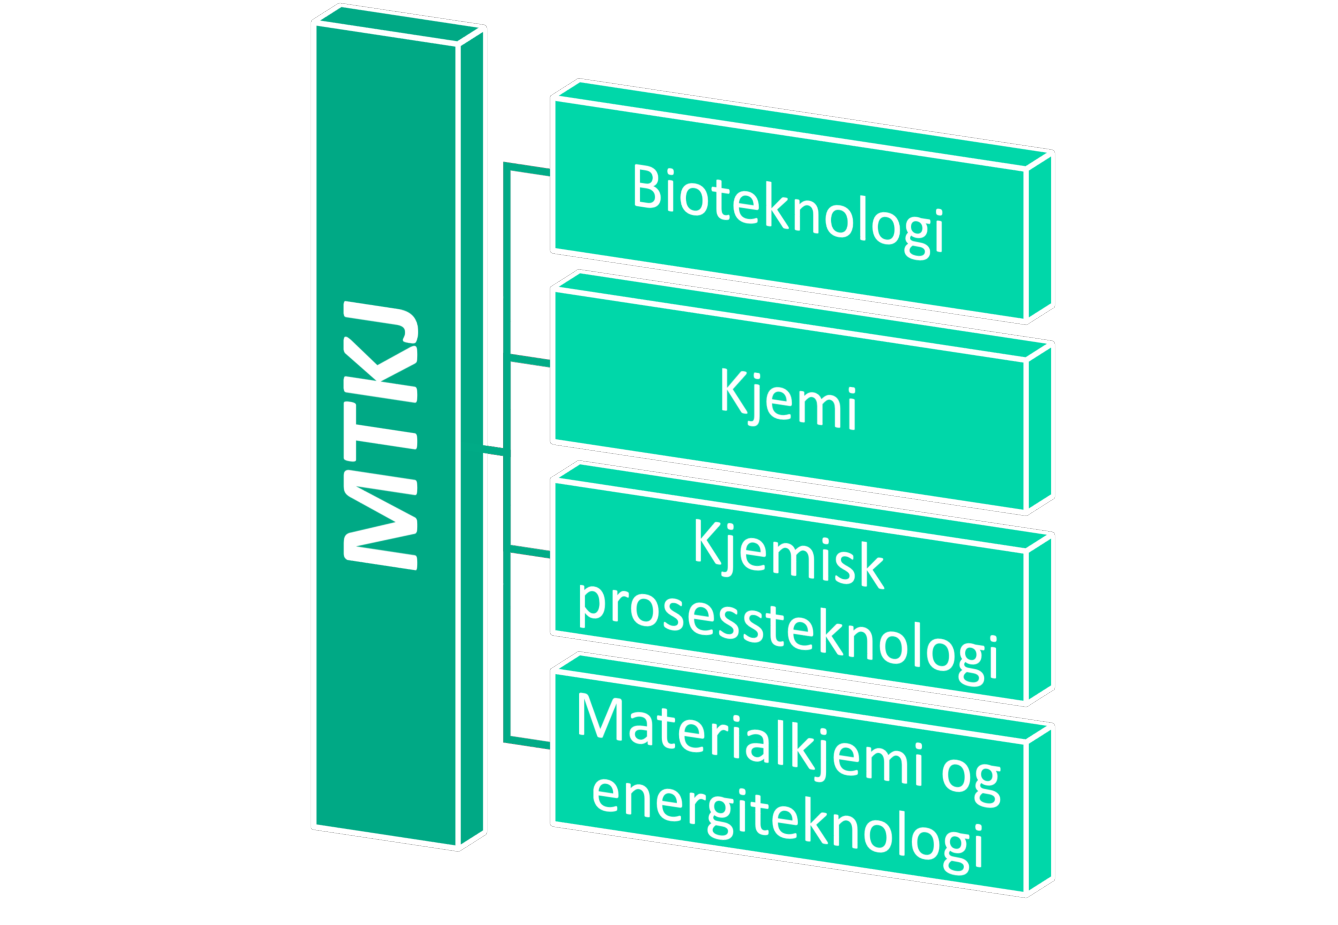
\includegraphics[width=0.8\textwidth]{images/Retningsvalg.pdf}
    \caption{De fire spesialiseringene man kan velge mellom}
    \label{fig:Spesialisering1}
\end{figure}

Valget av spesialisering må tas i løpet av høsten i 3. klasse. Tidligere valgte man spesialisering våren i 2. klasse, men dette ble forskjøvet med et semester fra og med kullet med oppstart i 2019. Det er heller ingen tilfeldighet at hver av spesialiseringene er knyttet til et eget institutt ved Fakultet for Naturvitenskap (NV). Man kan ofte høre prosessfolka snakke om IKP (Institutt for kjemisk prosessteknologi) eller mattek snakke om IMA (Institutt for materialteknologi).

Men hva i all verden er en \textit{hovedprofil}? Det er rett og slett det som kommer etter at man har valgt spesialisering. Dette valget skjer gjerne på et senere tidspunkt, i 4. eller 5. klasse. Det finnes unntak, som for eksempel i retningen \textit{kjemi}, hvor man allerede ved valg av spesialisering også velger hovedprofil (det som HP står for). En oversikt over de ulike hovedprofilene er vist i Figur \ref{fig:Spesialisering-Hovedprofiler}. Det er verdt å merke seg at disse hovedprofilene heller ikke eksisterer ved en tilfeldighet, men reflekterer de ulike forskningsgruppene innad i instituttet. Hvert institutt består ofte av fire forskningsgrupper som hver reflekterer deres fokusområder. Ved IKP finnes det eksempelvis en gruppe innen katalyse, men ikke biomedisin. 

\begin{figure}[H]
    \centering
    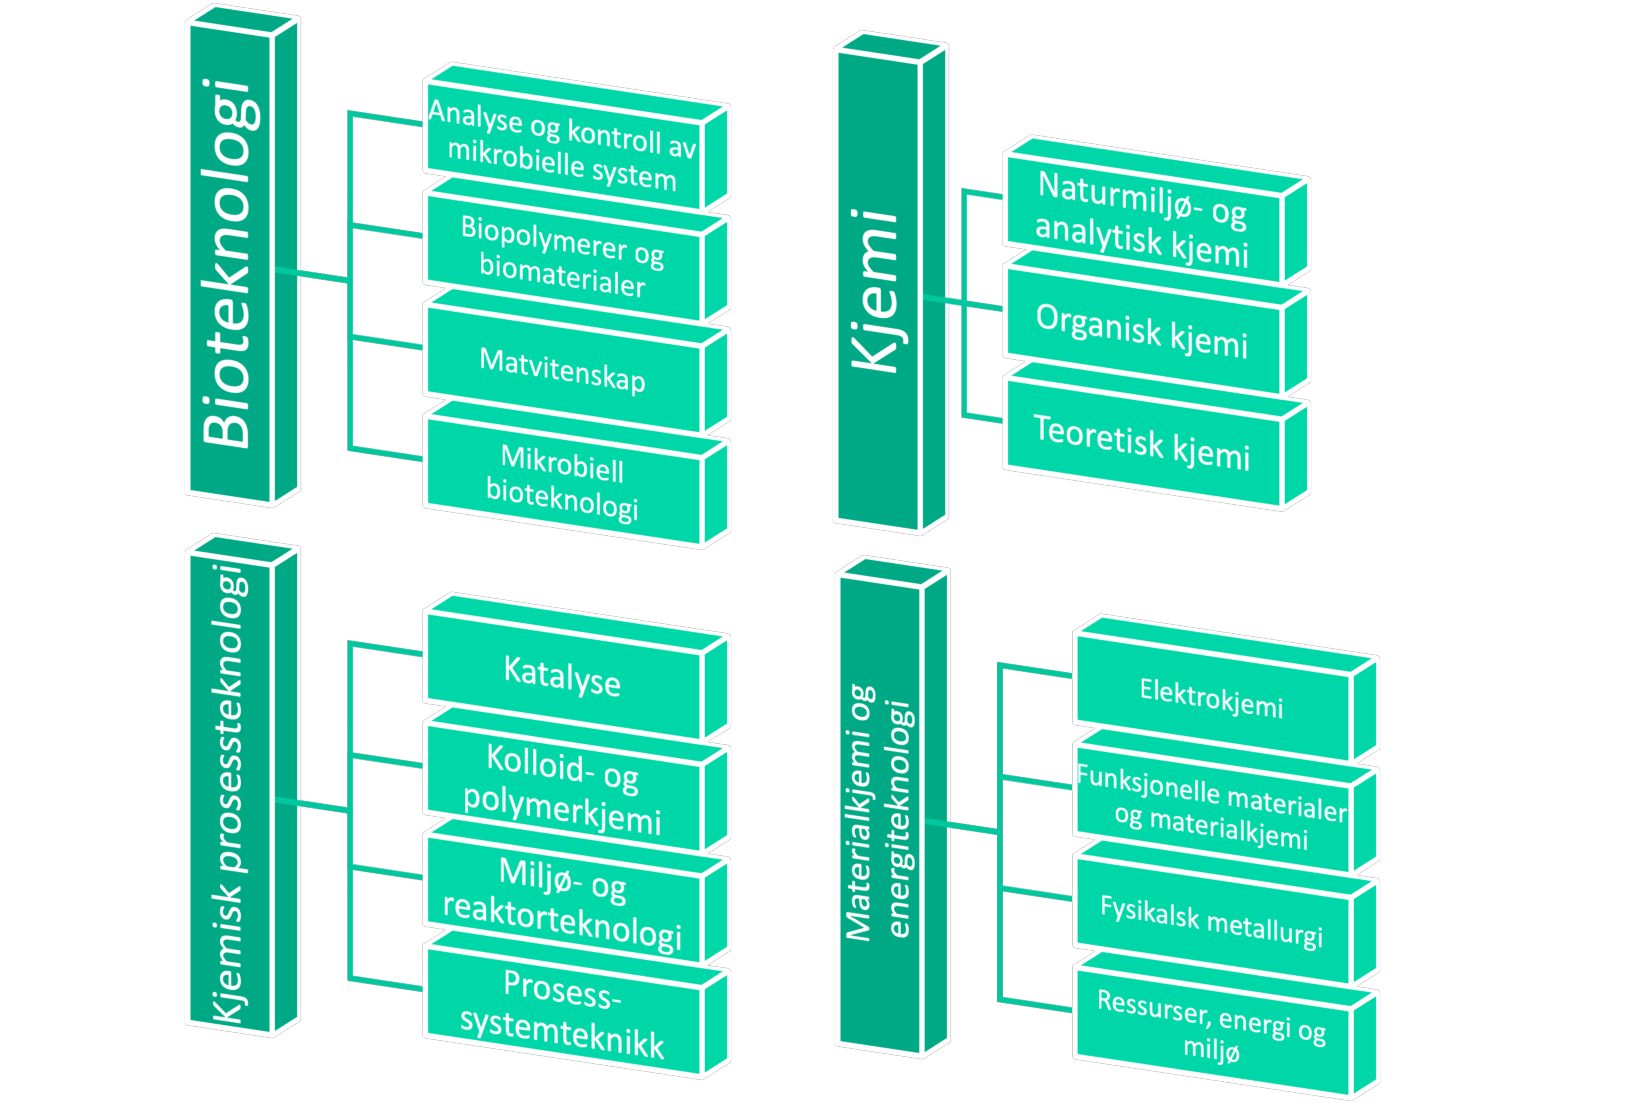
\includegraphics[width=0.9\textwidth]{images/Spesialisering-Retninger.pdf}
    \caption{Oversikt over de mange hovedprofilene man kan velge mellom.}
    \label{fig:Spesialisering-Hovedprofiler}
\end{figure}


\begin{figure}[H]
    \centering
    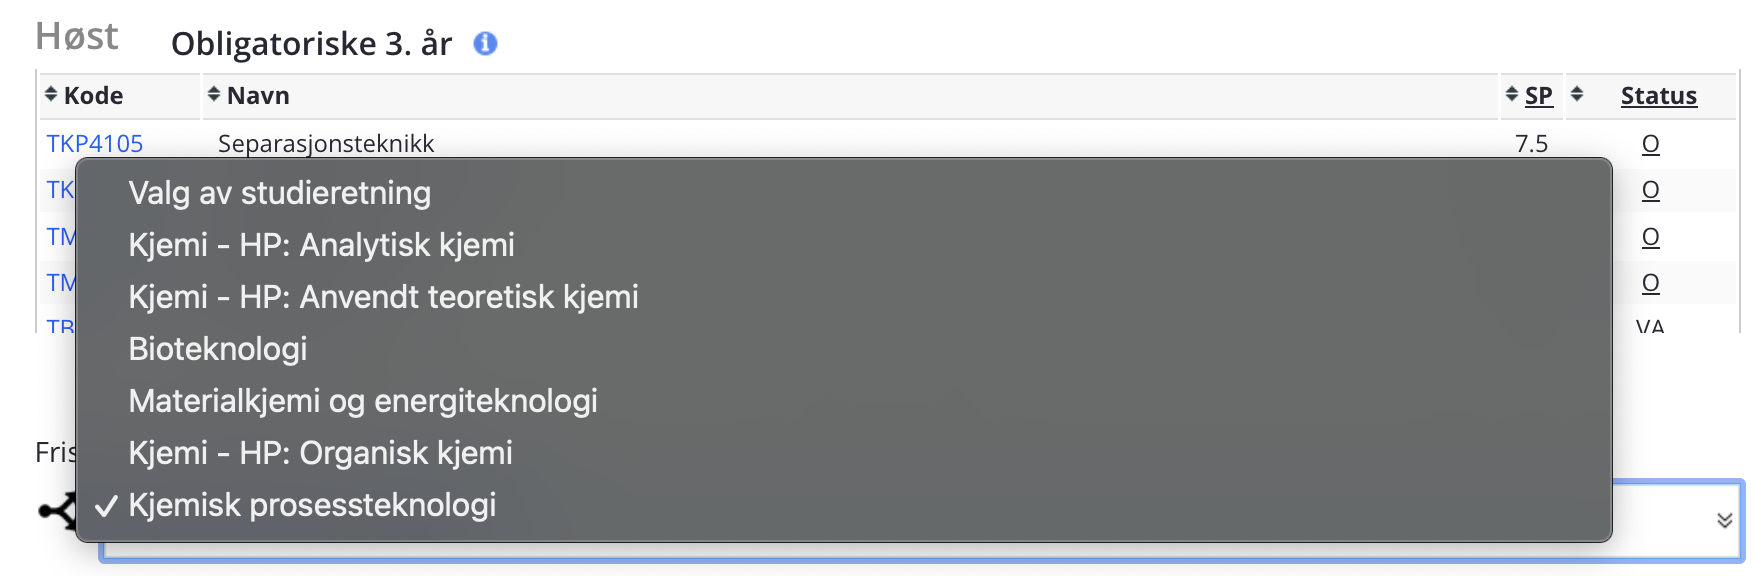
\includegraphics[width=1\textwidth]{images/spesialisering.png}
    \caption{Skjermbilde fra NTNU, dette burde være kjent ;)}
    \label{fig:Spesialisering-Screenshot}
\end{figure}


\section{Hvilken spesialisering bør jeg velge?}

Aha, dette spørsmålet har blitt stilt siden tidenes morgen. Det er et ganske ladd tema som jeg helst unngår å uttale meg om for å unngå heksejakt. Det jeg derimot kan anbefale, er å kikke gjennom listen med ulike ressurser:

\begin{enumerate}
    \item Snakk med en eldre chemiker (åpenbart)
    \item Dra på \textit{Livet etter Kjemi}
    \item \href{https://www.ntnu.no/studier/mtkj/studiets-oppbygning}{MTKJ-siden}
    \item Dra på spesialiseringsmøtene som blir avholdt før valgene
\end{enumerate}

Det er ikke alltid lett å vite hvilken spesialisering man skal velge, men hvis du er nysgjerrig, har jeg samlet en oversikt over spesialiseringene fra 2017-kullet (de som fullførte i 2022) til 2020-kullet (de som fullfører i 2025) i Figur \ref{fig:Spesialisering-Stolpe}.

\begin{figure}[!h]
    \centering
    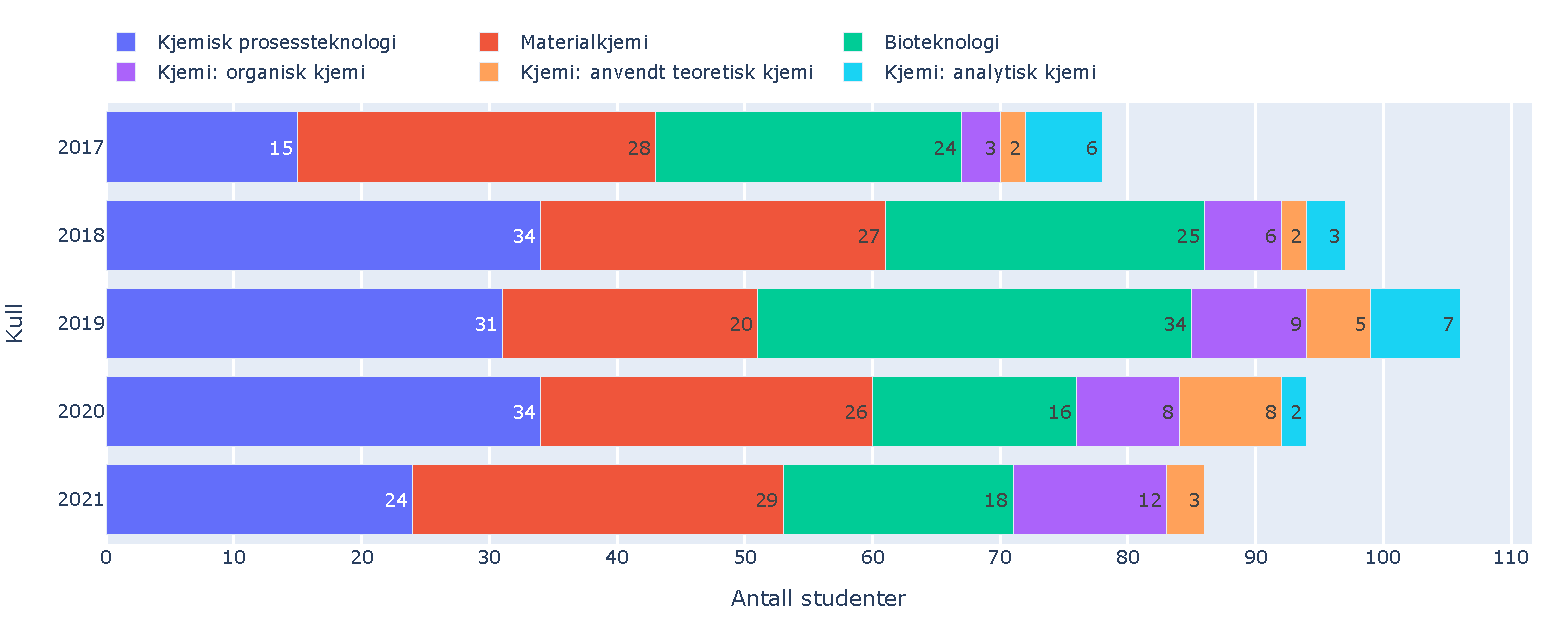
\includegraphics[width=1.1\textwidth]{images/Spesialisering_Stolpe.pdf}
    \caption{Fordeling av spesialisering fra 2017 til 2020-kullet, basert på startår\cite{Hege}}
    \label{fig:Spesialisering-Stolpe}
\end{figure}

Mange lurer spesifikt på jobbmuligheter og hvilke retninger som gir størst sjanse for å få jobb. Hvis du ser på Norges største industrier, er oljebransjen den mest kjente. Det er derfor svært mange muligheter om du jobber direkte i oljeselskaper eller i selskaper som på en eller annen måte har noe med olje å gjøre. I Norge er det også stor produksjon av metaller, typisk aluminium og silisium. Mye av fundamentet bak disse store industriene er kjemisk prosessteknologi og materialteknologi. Derfor er det enklest å få jobb innen disse retningene. Man kan argumentere for at bioteknologi er relevant for fiskeindustrien, men antall sysselsatte der er ikke i nærheten av olje- og metallindustrien. Når det gjelder organisk kjemi, kan man ende opp med arbeid overalt hvor det finnes laboratoriearbeid, men det avhenger igjen av hvor relevant jobben skal være – organisk syntese eller en laborant? Anvendt teoretisk kjemi minner mye om FysMat, og karriereveiene fører ofte til PhD eller konsulentjobb. 


\section{Hvordan ligner MTKJ på de andre studiene ved NTNU?}

Man vil merke at mange studier ved NTNU har flere fellestrekk, og at det til tider bare er en stor grøt med fag og fagfelt. Det kan være lurt å vite hvordan MTKJ ligner på de andre studiene på Gløs, slik at man eventuelt kan bruke dette til å lene seg mot en retning man interesserer seg for, eller finne enkelte fag du får lyst til å ta i løpet av studiet. Her går jeg gjennom alle siving-studiene på Gløs samt noen ekstra studier. 

\begin{table}[H]
    \centering
    \begin{tabular}{p{3cm}p{10cm}}
        \toprule
        Fagfelt & Fellesnevnere \\
        \midrule
        Bygg- og miljøteknikk & Ved å velge mattek kan man ende opp med å arbeide med betong og ulike byggmaterialer. Prosess kan rettes mot vann og avløp. Det er også mulig å bevege seg mot arktisk teknologi ved å velge organisk kjemi. \\
        
        Datateknologi & Vi har tross alt \textit{Informasjonteknologi, grunnkurs}, og noen velger å ta \textit{Prosedyre- og objektorientert programmering (C++)} senere. Den mest populære retningen er kunstig intelligens, hvor mange innen prosess skriver om maskinlæring. I forbindelse med dette kan fag som \textit{Kjemometri}, \textit{Multivariat dataanalyse og maskinlæring} og \textit{Statistisk læring} være nyttige. Man kan derfor lett skrive om maskinlæring uten å være datastudent, slik undertegnede gjør :) \\
        
        Elektronisk systemdesign og innovasjon & Det nærmeste vi kommer er signalbehandling innen prosess. Ellers har vi lite med kretser å gjøre. \\
        
        Energi og miljø & Her er det mye overlapp med en av spesialiseringene til EMIL-studentene. Deres spesialisering \textit{Energi- og prosessteknikk} har mange fellestrekk med prosess, og mange tar derfor \textit{Energiutnyttelse og prosessintegrasjon i industrielle anlegg}. Det skal sies at EMIL-prosess og MTKJ-prosess konkurrerer om de samme jobbene da begge faller under "prosessteknikk". \\
        
        Fysikk og matematikk & Vår kjære FysMat, her er det naturlig mange likheter. Liker du kvantekjemi eller termodynamikk, nærmer du deg spesialiseringen \textit{Teknisk fysikk}. Liker du modellering, optimalisering og statistikk, og velger disse mattetunge retningene i anvendt kjemi, mattek eller prosess, nærmer du deg \textit{Industriell matematikk}. Deres \textit{Biofysikk og medisinsk teknologi} kan minne om en bioretning på matte-steroider. Industrien ansetter også FysMat-studenter, men de fleste jobber heller i forskning eller som konsulenter. \\
        
        Georessurser og geoteknologi & Det nye navnet på sivilingeniørstudiet \textit{Petroleumsfag}, som minner mye om visse retninger innen prosess. Det er ingen hemmelighet at mange fra MTKJ, spesielt prosess, får jobb innen olje og gass. De har også fag som \textit{Prosessteknikk} og \textit{Separasjonsteknikk} som en del av fagplanen. \\
        \bottomrule
    \end{tabular}
    \caption{Hvordan MTKJ ligner på andre studier DEL 1}
    \label{tab:AndreStudierDel1}
\end{table}

\newpage

\begin{table}[H]
    \centering
    \begin{tabular}{p{3cm}p{10cm}}
        \toprule
        Fagfelt & Fellesnevnere \\
        \midrule
        Industriell design & Strengt tatt ikke et sivilingeniørstudie lenger, men om du har interesse for design og farger, kan \textit{Visuell formidling} være interessant. \\
        
        Industriell økonomi og teknologiledelse & Indøk har sine teknologiretninger som er de samme som mange av de nevnte studiene på denne listen, så det tekniske sier seg selv. Men om du er interessert i økonomi og ledelse utover det som blir gjennomgått i \textit{Teknologiledelse}, kan du ta \textit{Finans for teknisk-naturvitenskapelige studenter} eller ta et år ekstra på \textit{Samfunnsøkonomi – bachelor} (eller ta det samtidig som sivilingeniørstudiet, en vanlig praksis). \\
        
        Ingeniørgeologi & Det nye navnet til \textit{Tekniske geofag}, som ligner mye på \textit{Georessurser og geoteknologi}. \\
        
        Ingeniørvitenskap og IKT & Dette studiet er planlagt slik at man kan velge en teknologiretning og deretter fokusere mer på IKT-delen. Det som er fint med MTKJ er at man ikke nødvendigvis gir opp muligheten til å jobbe med IT. Forskjellen ligger i at I\&KT er litt mindre datatungt enn \textit{Datateknologi}, men de fleste ender likevel opp som utviklere/IT-konsulenter. \\
        
        Cybersikkerhet og datakommunikasjon & Tidligere kjent som Kommunikasjonsteknologi og digital sikkerhet. Lite overlapp, de ser på flyten til datapakker, vi ser på flyten til molekyler. \\
        
        Kybernetikk og robotikk & En del overlapp om man velger prosess. Da driver man med optimalisering og regulering. Fag som \textit{Prosessregulering} (Skogestad sin variant av \textit{Reguleringsteknikk}) og \textit{Optimalisering og regulering} er relevante. Anvendt teoretisk kjemi kan også ha en del overlapp. Hvis man tar \textit{Multivariat dataanalyse og maskinlæring}, vil man merke at mange i dette fagfeltet har bakgrunn fra kjemi, og at faget minner mye om \textit{Kjemometri}. \\
        
        Marin teknikk & De liker båter som frakter ting, vi liker båter som frakter våre ting. \\
        \bottomrule
    \end{tabular}
    \caption{Hvordan MTKJ ligner på andre studier DEL 2}
    \label{tab:AndreStudierDel2}
\end{table}

\newpage

\begin{table}[H]
    \centering
    \begin{tabular}{p{3cm}p{10cm}}
        \toprule
        Fagfelt & Fellesnevnere \\
        \midrule
        Maskin- og energiteknologi & Det nye rebrandede navnet til \textit{Produktutvikling og produksjon}, men likhetene med MTKJ forblir de samme. Maskin har en prosessretning, \textit{Bærekraftige og energieffektive systemer}, som har mange fellestrekk med MTKJ-prosess og EMIL-prosess, men de ser litt mer på væsker. Deres retning \textit{Produktutvikling og materialer} har likhetstrekk med mattek, men de fokuserer mer på de fysiske egenskapene enn de kjemiske. \\
        
        Materialteknologi & Likhetene er åpenbare, men forskjellene er litt vanskeligere å definere. Man kan karakterisere det rene materialteknologistudiet som bestående av to retninger: prosessmetallurgi og fysikalsk metallurgi. MTKJ-mattek inneholder betydelige mengder ren kjemi og prosessteknologi \cite{MTKJ-MTMT}. Ved endt mastergrad har begge kandidater tilsvarende kompetanse, men forskjellen ligger i mer dybdekunnskap for MTMT og mer breddekunnskap for MTKJ-mattek. \\
        
        Nanoteknologi & Noen få fellestrekk med mattek-retningen, men nano ligger et sted mellom fysikk og materialteknologi. Man kan se på nano som en enda mer spesifikk retning innen materialteknologi. Siden nano ikke er en stor greie i Norge, ender de fleste som konsulenter eller tar PhD. \\
        
        Bioteknologi & Man skulle tro bioteknologi 5-årig og MTKJ bio er det samme, men det er noen vesentlige forskjeller: \textit{MBIOT5 har både grunnleggende og videregående emner i celle- og molekylærbiologi som ikke inngår i MTKJ-BT, mens MTKJ-BT har flere kjemiemner og unike kjemiprosessemner.} De har mange like masterprosjekter (både på problemstilling og metodikk), men grunnutdanningen og spesialiseringen i høyere årskurs er betydelig forskjellig. \textit{MTKJ-BT er en unik utdanning i Norge og gir et godt grunnlag i kjemi, kjemisk prosessteknologi og bioteknologi. NMBU tilbyr en 5-årig sivilingeniør i kjemi og bioteknologi, men den har ingen kjemiprosessemner. Dette studiet har mer til felles med MBIOT5, men med mer kjemi og matematikk. MTKJ-BT kandidater er ettertraktet i norsk bioprosess og kjemisk industri.} \cite{MTKJ-MTMT} \\
        
        Kjemiingeniør og materialteknologi bachelor & Disse er bachelorversjonene av MTKJ og MTMT og vil derfor ligne svært mye. Det er verdt å understreke at bacheloringeniørprogrammene ofte har andre versjoner av sivilingeniørfagene og oppleves ofte som lettere. Likevel kan man med en bachelor søke over på 2-årig master og ende opp som sivilingeniør, likt som MTKJ/MTMT. Man vil også på papiret ha samme kompetanse, men det er forskjeller i grunnutdanningen. De kan ta MSCHEMBI og likevel bli sivilingeniør. \\
        \bottomrule
    \end{tabular}
    \caption{Hvordan MTKJ ligner på andre studier DEL 3}
    \label{tab:AndreStudierDel3}
\end{table}



\section{Den grusomme praksisen}

På Gløshaugen elsker vi historie og tradisjoner. Selv om vi nå går på NTNU, bærer vi med oss en arv fra NTH-tiden: kravet om relevant arbeidserfaring. Dette kan høres skummelt ut, men tanken bak er egentlig god – det gir verdifull praktisk erfaring under studiet. Dessverre er det opp til studentene å finne denne erfaringen selv, noe NTNU prøver å adressere med pilotordninger for EMIL-studenter. Praksisordningen stammer fra NTH, da sivilingeniørstudiene varte i 4,5 år \cite{Praksis45}. For å bli tatt opp ved NTH måtte man ha et halvt år med relevant arbeidserfaring. NTNU har fjernet dette opptakskravet, utvidet studiet til fem år, men beholdt kravet om praksis i løpet av studietiden. Hvorfor opptakskravet om praksis ble fjernet er ukjent, men det ryktes at NTNU ikke orket papirarbeidet som fulgte med.

Mange kjenner ikke til praksiskravet, så her er et sitat fra Innsida \cite{PraksisNTNU} som beskriver det. Det samme kravet gjelder for de 2-årige masterprogrammene, men de har kortere praksiskrav enn de 5-årige programmene.

\begin{center}
    \begin{minipage}{0.8\textwidth}
        \begin{outline}
            \textit{Det stilles krav om til sammen 12 ukers arbeidslivserfaring for studenter på det 5-årige masterstudiet, hvor korteste godkjennbare periode er 2 uker og jobben skal normalt tilsvare minimum en 50\% stilling. Minst 6 av disse ukene med arbeidslivserfaring skal være faglig relevant for det gitte studiet.}
        \end{outline}
    \end{minipage}
\end{center}

Mange gruer seg til å søke sommerjobber fordi man får mange avslag, og det kan være ubehagelig å skrive søknader – noe som er veldig forståelig. Hvis jeg kan komme med et trøstende tips, så er det følgende:

\begin{remark}
    \textbf{TIPS} Verken studieveileder, NTNU eller studentene tjener noe på å bli holdt igjen fra å skrive masteroppgaven på grunn av manglende praksis. Hvis man virkelig prøver å søke på sommerjobber og kan vise til mange nok avslag (f.eks. 15 avslagsbrev), vil NTNU sannsynligvis godkjenne det.
\end{remark}

Man kan jo lure på hva som definerer \textit{relevant arbeidserfaring}. Det er lettere å definere hva som er relevant enn hva som er irrelevant. For eksempel vil en sommerjobb hos Hydro ofte være relevant. Dette kan innebære å modellere prosesser eller vaske gulv – NTNU trenger ikke vite detaljene. Derimot er det vanskeligere å argumentere for at en kassejobb på Kiwi er relevant, men det går rykter om at noen har fått det godkjent. Noe som ofte glemmes, er at jobber som studentassistent også teller som relevant erfaring. Siden relevant arbeidserfaring er 6 uker med 37,5 timer per uke, tilsvarer dette 225 timer – noe som kan oppnås med litt over to studass-jobber. Tips til hvordan man skaffer seg studass-stillinger finnes lengre nede.

Jeg vil også sterkt anbefale sommerjobber generelt, da de fleste betaler betydelig bedre enn jobber som servitør (jeg har tall lengre nede for å støtte dette) og gir deg muligheten til å bruke det du har lært på skolen. For min del har det vært utrolig givende å se hvordan en varmeveksler ser ut i industrien og forstå viktigheten av det jeg har lært. Fordelen er at du kommer tilbake til studiene etter sommerjobben og kan sette mer pris på det vi lærer. Å være sivilingeniørstudent er teoretisk, men det er en grunn til at ingeniører ikke er rene matematikere eller fysikere – vi anvender prinsippene fra realfagene. Derfor kan det være vanskelig å sette pris på det man kan ved å bare være på NTNU og ikke ute i næringslivet.


\newpage
\chapter{Relevant erfaring} \label{ch:relevant_erfaring}

I denne delen skal jeg introdusere de ulike typene relevant erfaring man kan få, hvordan man skaffer dem og hvor man finner disse stillingene. Jeg har valgt å dele det inn i fem kategorier:

\begin{enumerate}
    \item Summer internship
    \item Winter internship
    \item Ferievikarer
    \item Deltidsjobb ved studiene
    \item Kurs og caser
\end{enumerate}

Dette er noe som allerede 1.-klassinger kan kikke på, fordi flere kurs og opplegg krever at man er tidlig i studieløpet. Ved å vite om dette på forhånd kan man unngå å gå på en smell senere.


\section{Summer intership}

Jeg kommer til å bruke navnene summer internship, internship og sommerjobb om hverandre. Kjært barn har mange navn, men summer internship høres mer fancy ut.

Det første du trenger å vite, er at summer internships lyses ut på typiske jobbsøkeportaler som Finn og LinkedIn. Ofte er selskapene ute etter studenter i 3. og 4. klasse på grunn av progresjonen i studiet. Dette handler både om kunnskapene man besitter og om når de kan ansette deg! Jeg deler summer internships inn i to kategorier: bedrifter som bruker det som ekstra arbeidskraft i sommerperioden og bedrifter som bruker det som en intervjuprosess.

Den første kategorien fungerer i praksis som vikariater, hvor studentene løser små oppgaver de faste ansatte ikke har rukket å gjøre. Sommerferien er ofte en tid de fleste tar ferie, og siden mange bedrifter har oppgaver de gjerne skulle ha utført selv, overlater de derfor dette til studentene.

Den andre kategorien gir studentene egne prosjekter, som for eksempel en kundecase i et konsulenthus eller utforsking av nye ideer. I disse stillingene produserer studentene i varierende grad noe nyttig for bedriften og det handler mer om å finne de aktuelle studentene for en fast stilling. Derfor er en internship-stilling perfekt for en slik bedrift her, ettersom det er en 2 måneder lang intervjuprosess, men med ingen forpliktelse om å ansette vedkommende etterpå. Husk at dårlige ansatte koster mer enn å ansette sommerstudenter.

Når det gjelder intervjuprosesser, finnes det mange ulike metoder som bedrifter benytter. De fleste krever et motivasjonsbrev, CV og ofte karakterutskrifter. Store selskaper som Equinor har lange og tidvis krevende prosesser, hvor man må gjennom CV-sjekk, evnetester, automatiske videointervjuer og eventuelt et avsluttende intervju. Mange lurer på hvilke spørsmål som blir stilt under intervjuene, men dette er vanskelig å forutsi. Automatiske videointervjuer har ofte standardiserte spørsmål, så hvis en venn har tatt det før, er spørsmålene sannsynligvis de samme. Dette er nyttig å vite, siden du har begrenset med tid til å svare når spørsmålene dukker opp. 

Jeg vil også påpeke at konsulentbransjen ofte har de mest utfordrende intervjuene, hvor de kan stille tilsynelatende absurde spørsmål. For eksempel kan du bli spurt: <<Hvor mange golfballer får plass i en Boeing 747?>> eller <<Hva er markedsandelen til iPhone i India?>>. Det kan virke skremmende, men såkalte <<Guesstimates>> blir mye enklere å håndtere med litt øvelse. Det finnes mange guider som kan hjelpe deg med å løse slike oppgaver, noe jeg vil gå nærmere inn på senere.

\begin{remark}
    \textbf{OBS OM FRISTER} Sommerjobber har varierende frister, så det er viktig å starte søknadsprosessen tidlig, gjerne i august. Konsulenthus har ofte tidlige frister, mens større kjemirelaterte stillinger kommer i september/oktober og våren. Opprett varsler på Finn og LinkedIn med søkeordene: \textit{summer intern}, \textit{summer internship}, \textit{sommerjobb ingeniør} og \textit{sommerjobb teknisk}. Mange stillinger har fortløpende opptak, så søk tidlig. Det anbefales å ikke ta for mye hensyn til fristene da mange stillinger har fortløpende opptak uten å nødvendigvis nevne det.
\end{remark}

Historisk sett har det vært vanlig å søke både fulltidsjobber og sommerjobber i løpet av våren. Det kan virke merkelig å ansette en student allerede i september for en jobb som ikke starter før juni, men bedriftene har blitt stadig mer ivrige etter å sikre seg de beste kandidatene så tidlig som mulig. Dette handler ikke nødvendigvis om å få tak i de mest akademisk dyktige, men heller om å finne de mest motiverte som søker tidlig. Nylig har noen selskaper presset søknadsfristene så langt frem at de gikk ut allerede i august, noe som mange synes er urimelig. Som respons truet linjeforeningen Abakus med å kutte samarbeidet med bedrifter som opererte på denne måten, noe som førte til at fristene ble flyttet tilbake til september/oktober.

Det som derimot ikke snakkes så høyt om, er at mange stillinger nå har fortløpende søknadsfrister. Det vil si at hvis du søker på den oppgitte fristen i annonsen, kan det allerede være for sent. Selskapet kan ha sendt ut tilbud til flere kandidater før søknaden din i det hele tatt blir vurdert. Jeg har selv opplevd dette med en sommerjobb jeg var svært interessert i, men ventet for lenge med å søke på. Derfor er det viktig å være oppmerksom på fristene og søke i god tid.

\begin{remark}
    \textbf{HVORDAN LAGE CV} Det finnes mange fine CV-maler på Word og Overleaf, bruk dem. Tekna har også en CV-bygger med søknadsbrev som jeg har brukt. Skaff deg også LinkedIn, mange HR-folk liker å kikke på profilene til folk her. Her kan man også få lagt inn det man eventuelt ikke får plass til på CV-en. Legg ved LinkedIn-profilen din på CV-en. Skal du være enda mer fancy kan du lage din egen nettside, har du klart ITGK klarer man fint å lese seg opp på det, men er kanskje for de spesielt interesserte. 
\end{remark}

Det er verdt å bruke tid på CV-en sin, men legg merke til at det oftest bare tar tid den første gangen. Når CV-en har blitt laget så er vedlikeholdsprosessen mye lettere. Jeg ville heller fokusert på å bruke mer tid på å søke på stillingene, og et typisk tips er å lese annonsen nøye. Alt er der for en grunn, uavhengig om du forstår deg på det eller ikke. Det var flere ting jeg ikke skjønte med annonsen før jeg startet i internshipet, men først da ga det mening. Eller så burde jeg bare gjort mer research, hvem vet. Jeg ville også brukt LinkedIn til å finne hvem som hadde tilsvarende stilling i fjor og spurt om tips, ettersom de ofte vet hvilke spørsmål som stilles og hva HR fokuserer på. 

\begin{remark}
    \textbf{BILDE ELLER IKKE?} Det er et evig spørsmål om CV-en skal inneholde et bilde eller ikke. I England er dette en no no, men jeg ville ha oppfordret folk til å ta med bilde. Sett deg selv i skoene til en i HR, det er mye lettere å huske et fjes enn en CV. I den anledning ville jeg anbefalt å dra på CV-fotografering med Kjemidagen eller Tekna, begge er gratis! Eller så kan man spørre folk som er flinke til å ta bilder, de i Promokom kan ofte stille opp på kort varsel ;)
\end{remark}

Jeg vil også understreke hvor raskt folk kan eliminere seg selv fra en stilling ved å tro at de ikke oppfyller alle kvalifikasjonene. Det er viktig å huske at mange av de oppførte <<kvalifikasjonene>> ofte er veiledende, og hvis du klarer å selge deg selv godt nok, har det mindre betydning om du ikke oppfyller hver eneste en. Jeg fikk for eksempel et internship i et selskap som jobber med vannkraft, til tross for at jeg ikke hadde noen forkunnskaper om vannkraft (svaret er ingenting). Dette viser hvor mye motivasjon og personlighet betyr.

Selv om en stilling er merket som forbeholdt 4. klassinger, bør du likevel søke – kanskje får du den, og i verste fall har du bare brukt litt tid på søknaden. Hvis du er så heldig å få et internship tidlig og lurer på om det er verdt å søke i 4. klasse, er svaret mitt: absolutt! Som 4.-klassing blir du automatisk prioritert høyere enn 3.-klassinger, ikke nødvendigvis på grunn av mer erfaring, men fordi du er nærmere ferdig. For en arbeidsgiver fungerer et internship ofte som et forlenget intervju, og det er vanlig praksis i mange selskaper å tilby fast jobb eller deltidsjobb etter endt internship. Derfor bør du virkelig prioritere å søke internships i 4. klasse, for da har du kanskje sikret deg en fast jobb allerede før 5. klasse. Dette er en svært vanlig praksis blant konsulenthus, og litt mindre vanlig hos kjemibedrifter.




\section{Winter internship}

Ikke tro at sommerferien er den eneste perioden hvor du kan få internship! Selv om sommerferien er tiden hvor de fleste har fri, er det også vanlig med <<Winter internships>> rundt januar/februar. For mange bedrifter er dette faktisk mer gunstig, siden alle ansatte er på jobb, noe som gjør det lettere å følge opp studentene. Om sommeren kan ferieavvikling skape utfordringer, og derfor er noen bedrifter mer usikre på å tilby sommerjobber, fordi de må ha folk tilstede for å veilede studentene. Dette er vanlig praksis i konsulentbransjen, men mindre utbredt i industrien. Det betyr imidlertid ikke at mulighetene ikke finnes – ta kontakt med ansatte i bedriftene du er interessert i og spør om mulighetene!

Winter internships kan også være svært gunstige hvis du planlegger utveksling på våren, spesielt hvis semesteret er litt annerledes. For eksempel starter vårsemesteret i Italia i slutten av februar med eksamensperiode i juni/juli. Da kan det være vanskelig å få sommerjobb, men det gir en perfekt mulighet til å jobbe i januar/februar. Dette kan også åpne dører til flere muligheter senere. 


\section{Ferievikarer (perfekt for 1.klassinger!)}

Internships er ofte rettet mot studenter som har kommet et stykke ut i studiet, men det mange ofte glemmer er muligheten til å bli \textit{ferievikar}. Dette er stillinger som ikke nødvendigvis krever at man har kommet langt i studieløpet. Jeg tenker spesielt på stillinger som operatør hos bedrifter som Hydro, Elkem, vann- og avløpsetater, og lokale industriselskaper. Mange av disse stillingene er såpass enkle at selv videregående elever kan klare dem. For eksempel ansetter Hydro rundt 600 ferievikarer over hele Norge. Disse stillingene er godt betalt, på nivå med deres summer internships, og de blir godkjent som relevant erfaring.

Det som gjør MTKJ-studenter spesielt ettertraktede er vår solide forståelse for teknologi, grunnleggende prosesskunnskap, og kjemi. Dette gjør ferievikarstillinger hos Hydro til en perfekt mulighet for alle MTKJ-studenter.

Personlig angrer jeg veldig på at jeg ikke visste om denne muligheten tidligere. Som østlending hadde det vært utrolig spennende å for eksempel flytte til Vestlandet for en sommer, samtidig som jeg hadde hatt en interessant og relevant sommerjobb. 

\begin{figure}[H]
    \centering
    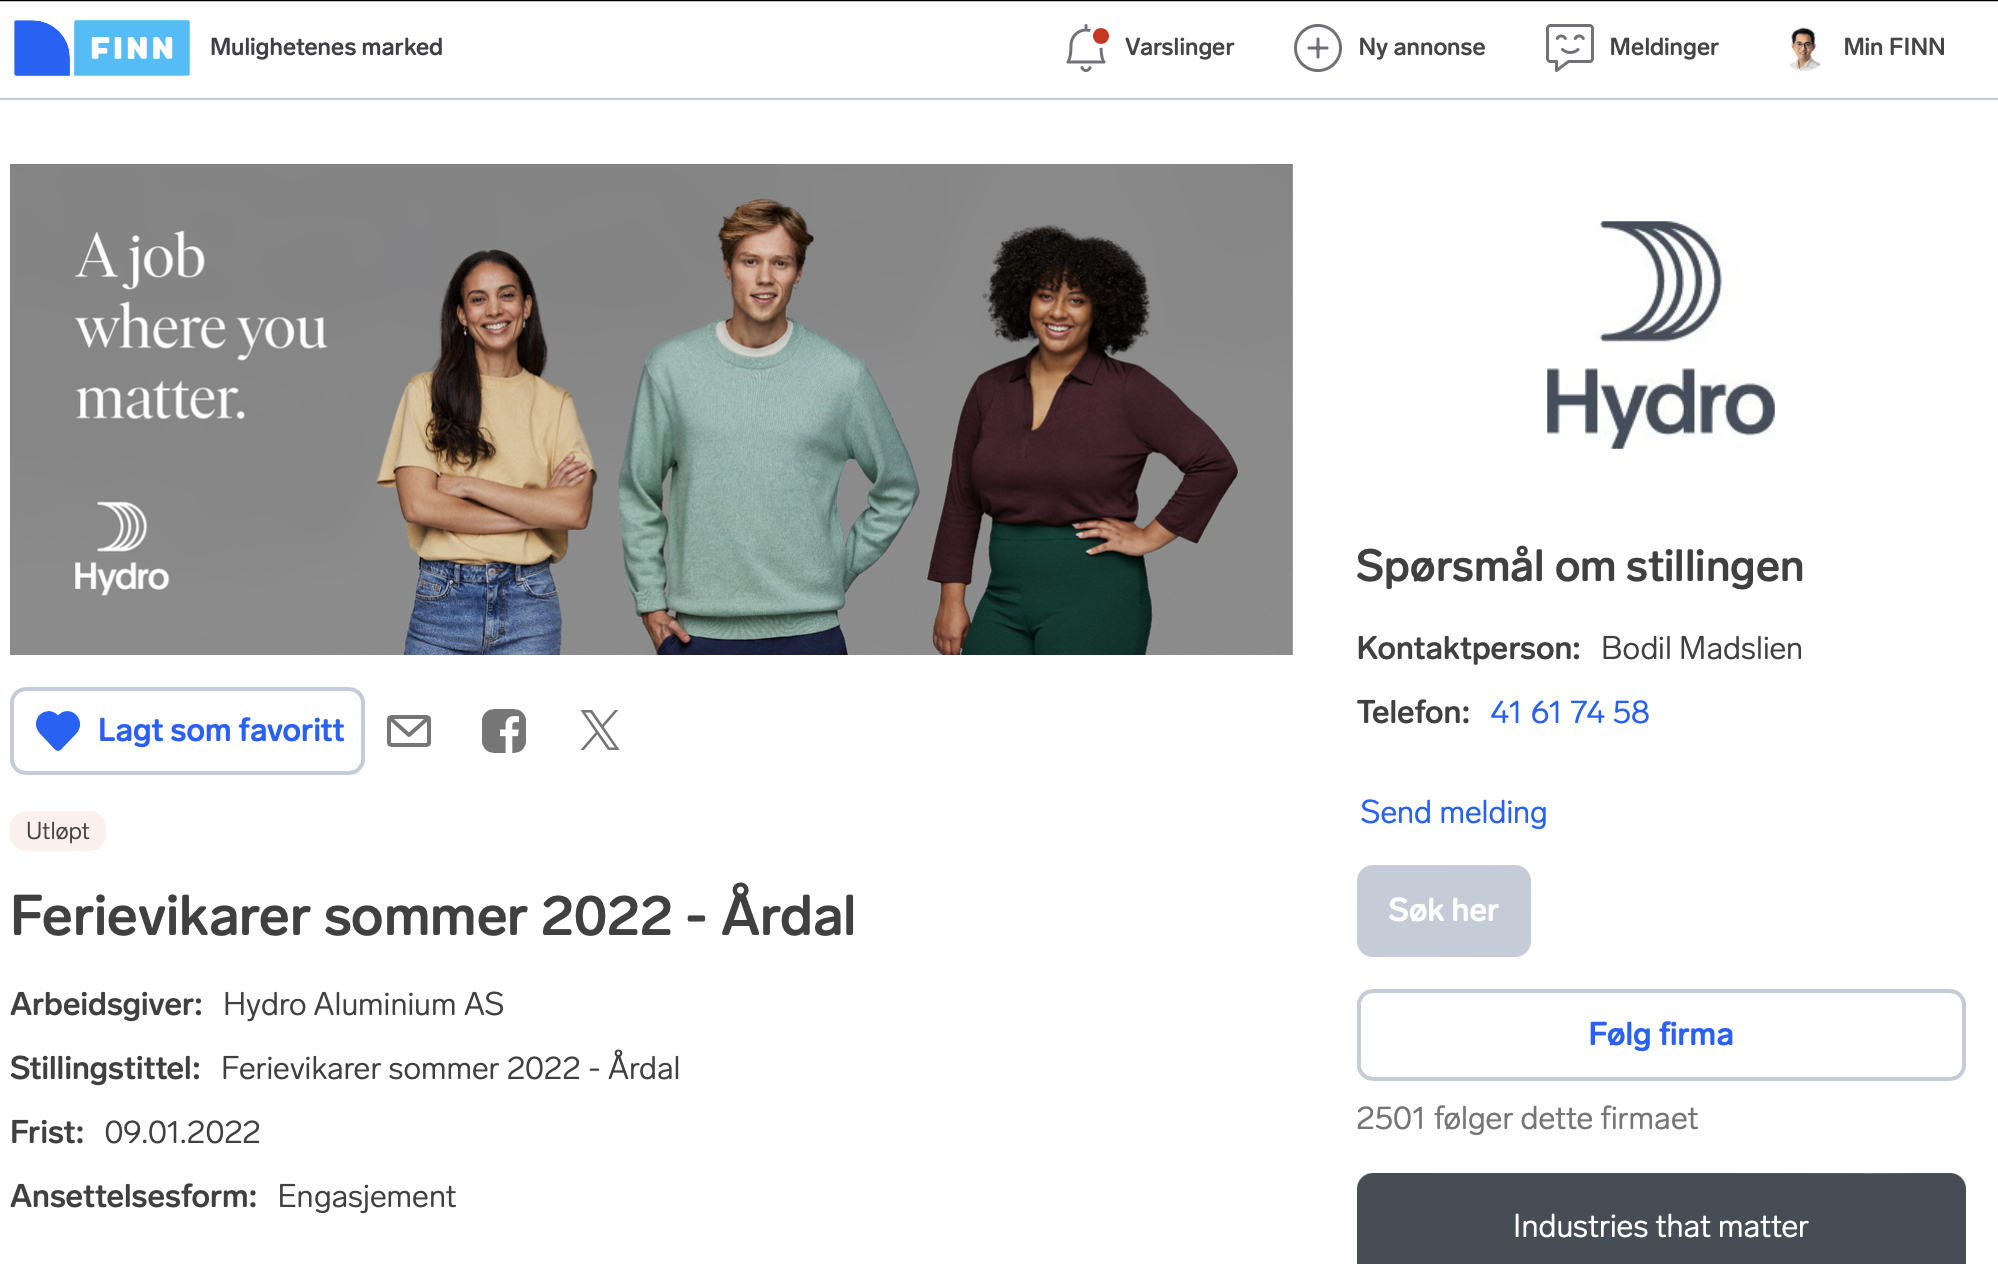
\includegraphics[width=1\linewidth]{images/hydro.png}
    \caption{Ferievikarstilling fra Finn.no}
    \label{fig:Hydro-annonse}
\end{figure}


\section{Deltidsjobb ved studiene}

De enkleste deltidsjobbene å få er ofte hos NTNU. Hvis du er interessert i å bli labassistent, kan du spørre foreleserne om de trenger hjelp i laboratoriet. For dem er det ofte billigere å bruke en student enn å sette en PhD-student på oppgaven. Dette kan føre til både en deltidsjobb under studiene eller en videreføring til en sommerjobb.

Den aller enkleste måten å få en deltidsjobb på, er å bli studassistent. Det er en myte at du må ha A i faget for å bli studass. Det handler mer om å være strategisk. Ja, hvis mange søker på stillinger i Generell kjemi, blir det ofte A-studentene som får jobbene, men husk at det finnes mange andre kjemifag. Flere sivilingeniør- og ingeniørstudier har kjemi eller basisfag som en del av pensum. Da kan det for eksempel holde med en C for å bli studass for byggstudenter. Du kan også bli studass i forkurs, som dekker grunnleggende videregående kjemi. Derfor anbefaler jeg at du ser gjennom alle studass-stillingene – det finnes alltid noen stillinger som ansetter bredere. Ikke alle fag har studass-opplegg på nivå med ITGK og matte.

Det er også viktig å få din første studass-stilling. Alle som blir studass må ta et kurs ved NTNU som heter LAOS-kurset. Når du har tatt dette kurset, blir det lettere å få din neste stilling, siden de ikke trenger å betale deg like mye som søkere uten LAOS-kurs. Du kan også få LAOS-kurs ved å være Teknostart-studass, så det er absolutt verdt å søke der også.



\section{Kurs og caser}

Dette er min favorittkategori fordi det rett og slett er gøy. Det kan virke litt overambisiøst å lete etter kurs eller casekonkurranser og deretter søke på dem, men la oss ta en titt på hva det egentlig handler om.

La oss begynne med kurs. Det finnes utallige kurs du kan søke på. NTNU har mange samarbeid med utenlandske universiteter, noe som gir deg muligheten til å få finansiert for eksempel en uke med studiepoenggivende kurs i Hellas. I tillegg finnes det kurs arrangert av bedrifter, som Bearingpoints konsulentskole. Hvis du er jente (som de fleste på MTKJ er), kan du også prøve deg på McKinseys program rettet mot unge kvinner.

\begin{figure}[H]
    \centering
    
\includegraphics[width=1\linewidth]{images/bearingpojnt.png}
    \caption{Bearingpoint som konsulentskole, verdt å kikke på}
    \label{fig:Beairngpoint}
\end{figure}

\begin{figure}[H]
    \centering
    
\includegraphics[width=0.8\linewidth]{images/mckinsey.png}
    \caption{Women Leadership Program}
    \label{fig:enter-label}
\end{figure}

Nå skal jeg snakke spesifikt om casekonkurranser. Disse kan ofte oppfattes som slitsomme, men det er egentlig ikke tilfellet! En typisk casekonkurranse går ut på at man får begrenset med tid til å løse et problem som ofte virker umulig. Det handler imidlertid mer om å tenke utenfor boksen og vise juryen hvordan din løsning er unik – du trenger ikke nødvendigvis å finne opp en ny kreftmedisin, liksom. 

Men la oss være ærlige, man deltar ikke på casekonkurranser bare for moro skyld, men også for fordelene de gir. Så hva er det egentlig man kan få ut av det? Jeg skal liste opp noen av disse konkurransene og hvilke goder de tilbyr i Tabell \ref{tab:Casekonkurranser}. Det finnes mange flere, men dette er de jeg har mest erfaring med.

\begin{table}[H]
    \centering
    \begin{tabular}{p{3cm}p{10cm}}
        \toprule
        Event & Innhold \\
        \midrule
        Aker Talent & Reise tur-retur Oslo inkludert hotellopphold, mat (+ drikke hehe), og sosialt opplegg som curling. Varer i 2 dager. Premien er litt uklart da det varierer fra år til år, men svært mange blant deltagerne får tilbud om sommerjobb eller fulltidsjobb fra et av Aker-selskapene (og det er heldigvis mange!). \\
        
        Skanska Grensesprenger & En av de lengre casene hvor man lager et lag selv og løser oppgave på egen tid. Premien er derimot ganske syk, fordi de sletter studielån opptil 165 000 kr for alle på vinnerlaget. \\
        
        Norconsult Hunger Games & Høres weird ut, men faktisk ganske artig med ulike aktiviteter osv. Det er hovedsakelig bygg, EMIL og maskinstudenter, men som MTKJ har man muligheten til å skille seg ut. Det foregår på kveldstid over to dager i Trondheim så ikke like intenst som andre. Det er selvfølgelig middag og drikke inkludert. Man blir heldigvis eliminert i puljer, så man ikke trenger å føle seg dårlig (jeg røk ut i første pulje). Vinneren får tilbud om fulltidsjobb hos Norconsult. Det du derimot ikke får vite, men som er svært viktig, er networkingen som skjer underveis. Det er 50 deltagere og like mange representanter fra Norconsult tilstede. De gjør ikke dette fordi penger er lættis, men fordi de er ute for å kikke etter folk. Dette gjør at noen kan ryke ut første runde, men likevel få sommerjobb den neste uken bare av å snakke med folk. \\
        
        Clara Idéathon & Du blir flydd til Bergen med hotell og alt sammen, ligner veldig på Aker Talent. Clara var derimot mindre skummelt siden det ikke var like mange tilskuere som på Aker Talent. \\
        
        Kongsberg Your Extreme & En konkurranse som arrangeres av Kongsberg ved NTNU og USN (Kongsberg, duh). Premien er på 100 000 kr , og det fine her er at alle deltagere blir invitert til en gallamiddag på Scandic Lerkendal. Så worst case er en 3-retters middag. \\
        
        AF-kollektivet & En årlig konkurranse hvor premien er å bo gratis i et år. Det huset vinnerlaget får er ganske gigantisk, så det er absolutt verdt tiden man investerer. \\
        \bottomrule
    \end{tabular}
    \caption{Oversikt over noen casekonkurranser}
    \label{tab:Casekonkurranser}
\end{table}

\begin{figure}[H]
    \centering
    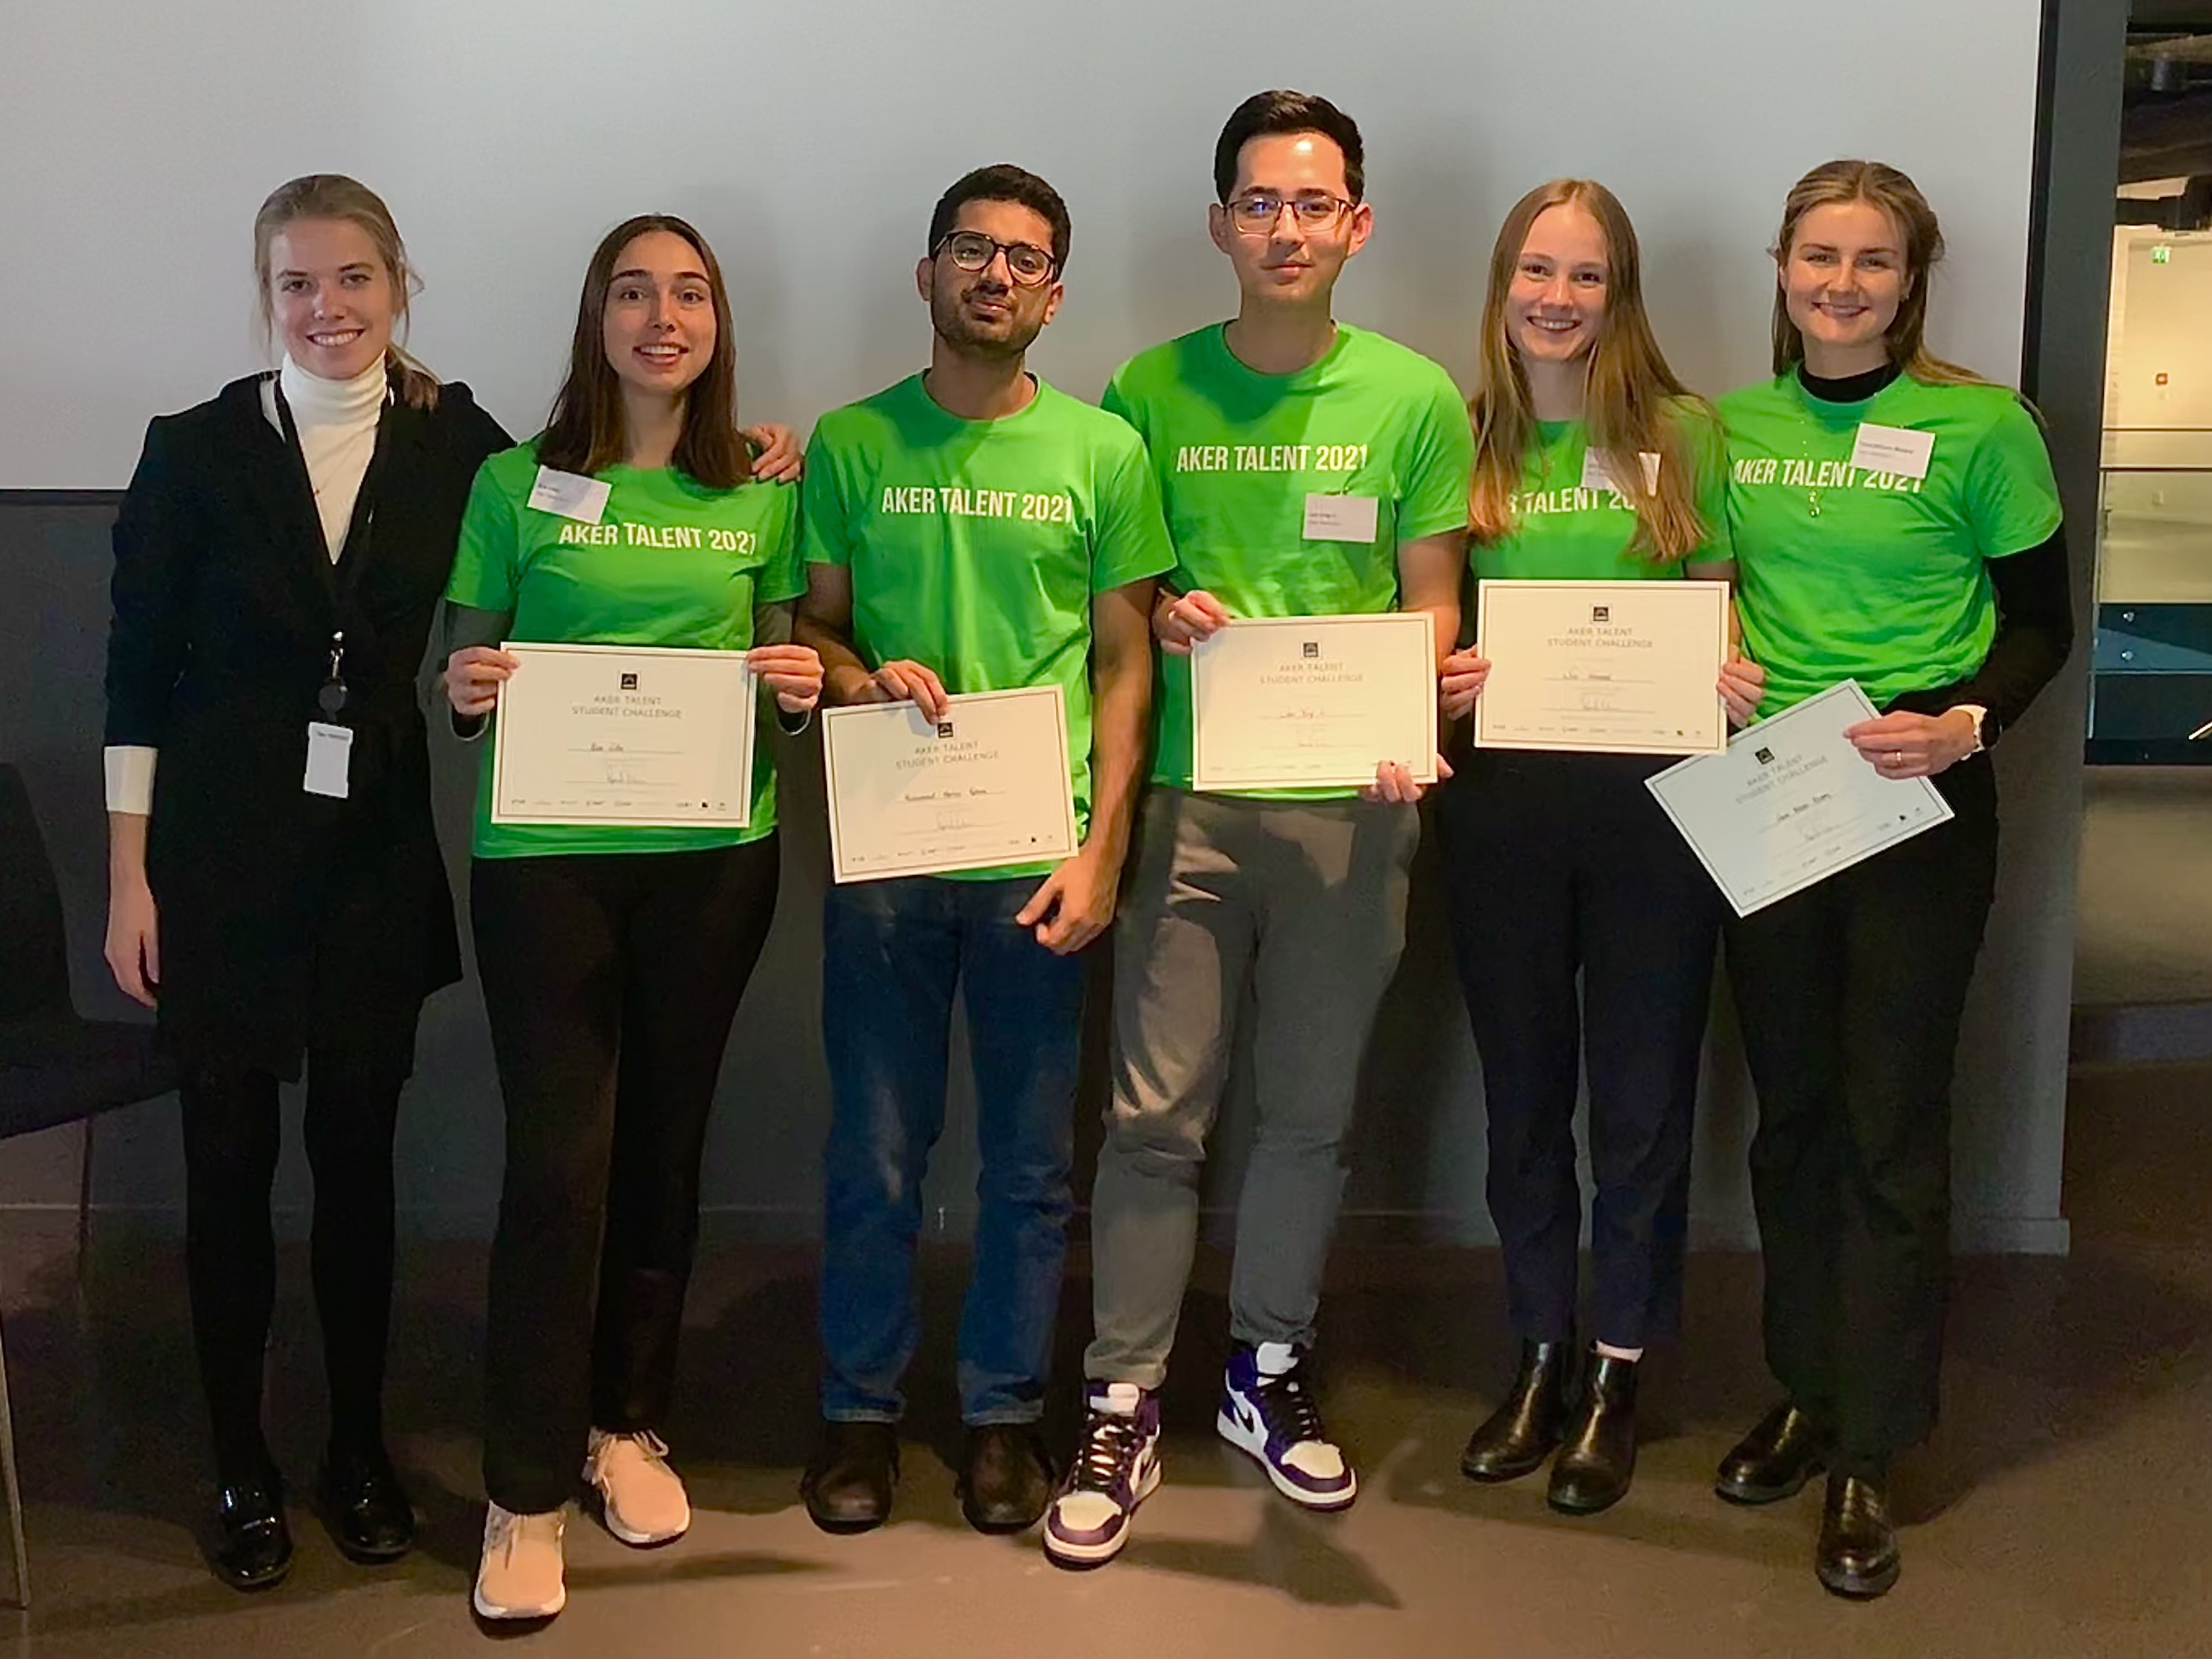
\includegraphics[width=0.6\linewidth]{images/Aker.jpg}
    \caption{Xing på Aker Talent, han høyeste med Jordans.}
    \label{fig:Aker}
\end{figure}

\begin{figure}[H]
    \centering
    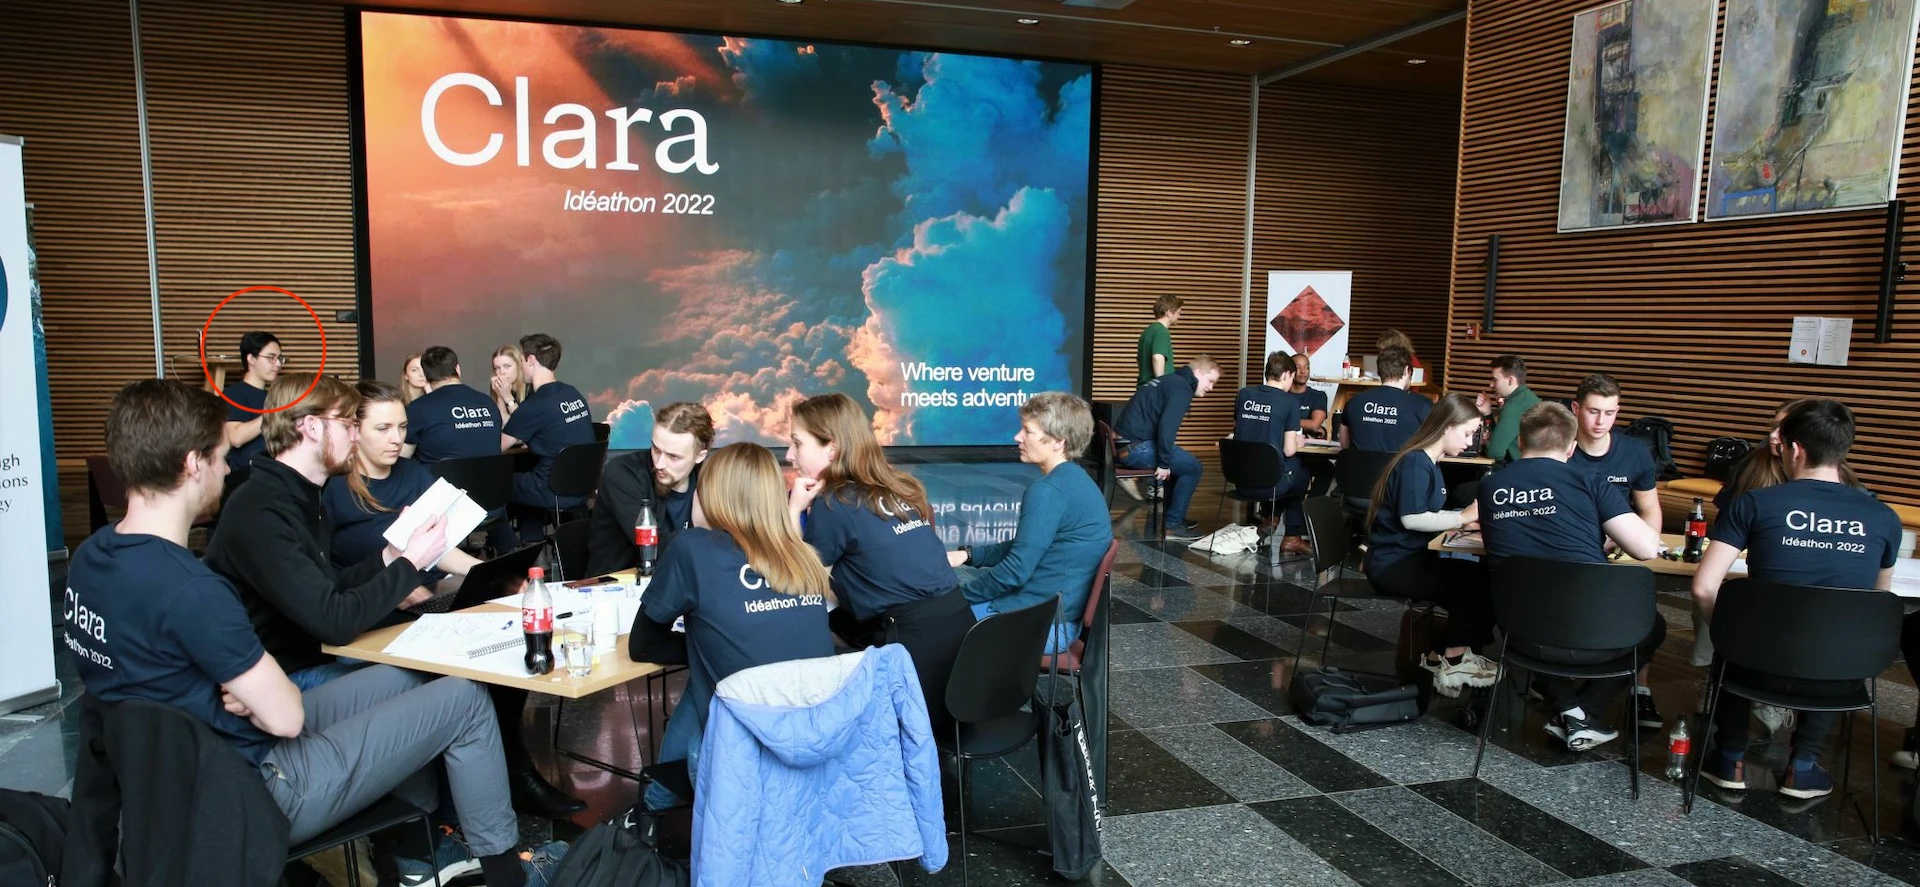
\includegraphics[width=0.8\linewidth]{images/Clara.jpg}
    \caption{Xing på Clara Idéathon, rød sirkel.}
    \label{fig:Clara}
\end{figure}



\newpage
\chapter{Jakten etter bedpres} \label{ch:bedpres}
For de som kjenner meg, vet dere at bedpres er en av mine hjertesaker. Nå skal jeg dele mine beste tips for hvordan DU kan bli en \textbf{\large Bedpres Hunter}.

\begin{figure}[H]
    \centering    
    
\includegraphics[width=0.7\linewidth]{images/BedpresHunters.jpg}
    \caption{Jeg brukte mange timer på plakaten, så jeg må vise den fram når jeg har muligheten ;)}
    \label{fig:bedpres}
\end{figure}




\section{Hva er bedpres?}

Hvis du aldri har hørt om ordet <<bedpres>>, så er det en forkortelse for \textit{bedriftspresentasjon}. Det er viktig at det ikke skrives som <<bedpress>>, som noen gjør. En typisk bedpres består av følgende deler:

\begin{itemize}
    \item Presentasjon av bedriften (ca. 1 time)
    \item Bespisning 
    \item Dra ut på byen (avhenger av bedrift)
\end{itemize}

Ingen bedpres er like og de vil derfor variere veldig. Noen kan tilby Pizzabakeren, mens andre kan tilby 3-retters middag med vinpakke og åpen bar på Downtown etter måltidet. 




\section{Hvorfor bedpres?}

Det er to grunner for å dra på bedpres: bli kjent med bedriften og gratis mat/drikke. Jeg drar utelukkende for det sistnevnte, men som en konsekvens så har jeg blitt kjent med ganske mange bedrifter. Nå skal jeg ramse opp en rekke bedpreser jeg har dratt på for å vise frem hva man kan forvente av slike arrangementer.

\begin{table}[H]
    \centering
    \begin{tabular}{r p{10cm}}
        \textbf{Bedrift} & PwC \\
        \textbf{Når} & Høsten 2022\\
        \textbf{Arrangør} & HC og Nabla\\
        \textbf{Oppsummering} & Ulike aktiviteter på kontoret deres i Trondheim, gruppen min vant konkurransen og fikk et handlenett med vannflaske og JBL høyttaler hver. Det var wraps og drikke under presentasjonene. Etter opplegget var det mingling og vi tømte øltappen på kontoret (ja de har øltapp på kontoret). Etter det dro vi til Solsiden og fikk spandert pizza-og pastabuffet pluss to enheter på Una Pizzeria.\\
        & \\
        \textbf{Bedrift} & Boston Consulting Group (BCG)\\
        \textbf{Når} & Høsten 2023\\
        \textbf{Arrangør} & Bindeleddet\\
        \textbf{Oppsummering} & 3-retters middag med vinpakke på Jossa (en del av Credo) og åpen bar. Undervies var det en del presentasjoner og artig underholdning. Etter middagen gikk bussen videre til Downtown (DT-torsdag altså) og der var halve 2.etasje reservert med åpen bar.\\
        & \\
        \textbf{Bedrift} &  BearingPoint\\
        \textbf{Når} & Høsten 2022\\
        \textbf{Arrangør} & Bindeleddet\\
        \textbf{Oppsummering} & Presentasjonen foregikk på Kjelhuset, før det etterpå endte på Søstrene Karlsen for en 3-retters middag. Det var åpen bar, men ikke godt egnet på en mandag ;)\\
        & \\
        \textbf{Bedrift} & Nammo Raufoss \\
        \textbf{Når} & Våren 2024\\
        \textbf{Arrangør} & Teknologiporten\\
        \textbf{Oppsummering} & Presentasjon i S8 på Stripa. Grunnet omstendighetene ble vi møtt av demonstranter som oppfordret til å boikotte bedpresen. For å unngå prikk så dro de fleste likevel og etter presentasjonen endte vi opp på Graffi Solsiden med burgermiddag og to enheter.\\
    \end{tabular}
    \caption{Oversikt over noen bedpreser.}
    %\label{tab:Casekonkurranser}
\end{table}




\section{Hvordan bedpres?}

Det finnes mange måter å komme seg inn på bedpreser. Jeg holder meg til tre kanaler:
\begin{enumerate}
    \item HC Industrikomiteen
    \item Teknologiporten
    \item Bindeleddet
\end{enumerate}

HCs \textbf{Industrikomite} har ansvar for å arrangere bedpres for medlemmer av linjeforeningen. Bedpresene er derfor alltid relevante for deltakerne, siden bedrifter spesifikt signerer avtaler med HC.

Deretter har vi \textbf{Teknologiporten} (TP), et samarbeid mellom flere studier ved Fakultet for Ingeniørvitenskap (IV – vi er NV). Her arrangeres det flere bedpreser i uken, mens HC kanskje har én i måneden. Som medlem av HC er man ikke blant de "utvalgte" ved TPs arrangementer, så det er viktig å sende en mail til den ansvarlige og spørre om MTKJ kan bli invitert. HC får penger fra TP for deltakelse på arrangementer, så jeg oppfordrer gjerne folk til å dra.

Man kan spørre hvorfor HC ikke er en del av TP, og jeg mistenker det handler om historie og misforståelser rundt kjemi. HC var ikke med da ønsket om å grunnlegge TP ble fremmet, og derfor kan de gatekeepe, fordi det ligger økonomiske interesser bak. En annen grunn er at mange misforstår hva vi egentlig studerer – vi blir ikke kjemikere, men kjemiingeniører. Som jeg nevnte tidligere da jeg snakket om spesialiseringene våre og hvordan vi ligner på andre studier, er ikke TP klar over dette og de ser derfor på oss som likestilte med \textit{Volvox og Alkymisten} (linjeforeningen for biologi- og kjemistudenter). Til tross for utfordringene, kommer man langt med en hyggelig mail, noe jeg har gjort for å få med MTKJ på flere bedpreser.

Den siste kanalen er det beryktede \textbf{Bindeleddet}, som drives av indøk-studenter. De markedsfører seg som bindeleddet mellom bedrifter og studenter ved NTNU, men de sitter igjen med all inntekten (som kan være i millionklassen). Som en konsekvens blir ofte MTKJ og andre studenter invitert til deres arrangementer. Bindeleddet sine bedpreser er de mest ekstreme, med åpen bar, 3-retters middager, og gjesteopptredener fra kjendiser. Det er også lettest å delta på bedpres via Bindeleddet, som ofte har tre bedpreser i uken. Etterspørselen etter å holde bedpres hos Bindeleddet er så høy at plassene for neste semester <<selges ut>> i løpet av timer etter at de har åpnet (angivelig).


% =======================================================================================
%                                   PART II
% =======================================================================================
\part{Karriereveier}
%----------------------------------------------------------------------------------------
\newpage
\chapter{Hvordan finne jobber}
\section{Oversikt over verktøy}

Det er en egen kunst å finne relevante stillinger, enten det gjelder internships, deltidsjobber eller faste stillinger. I dette avsnittet vil jeg introdusere noen nyttige verktøy for prosessen, og hvordan du bruker de riktige søkeordene på ulike plattformer. Nøkkelen ligger i å optimalisere søkene dine, og etter mye prøving og feiling har jeg kommet frem til noen konklusjoner som jeg vil dele i de påfølgende avsnittene.

\begin{figure}[H]
    \centering
    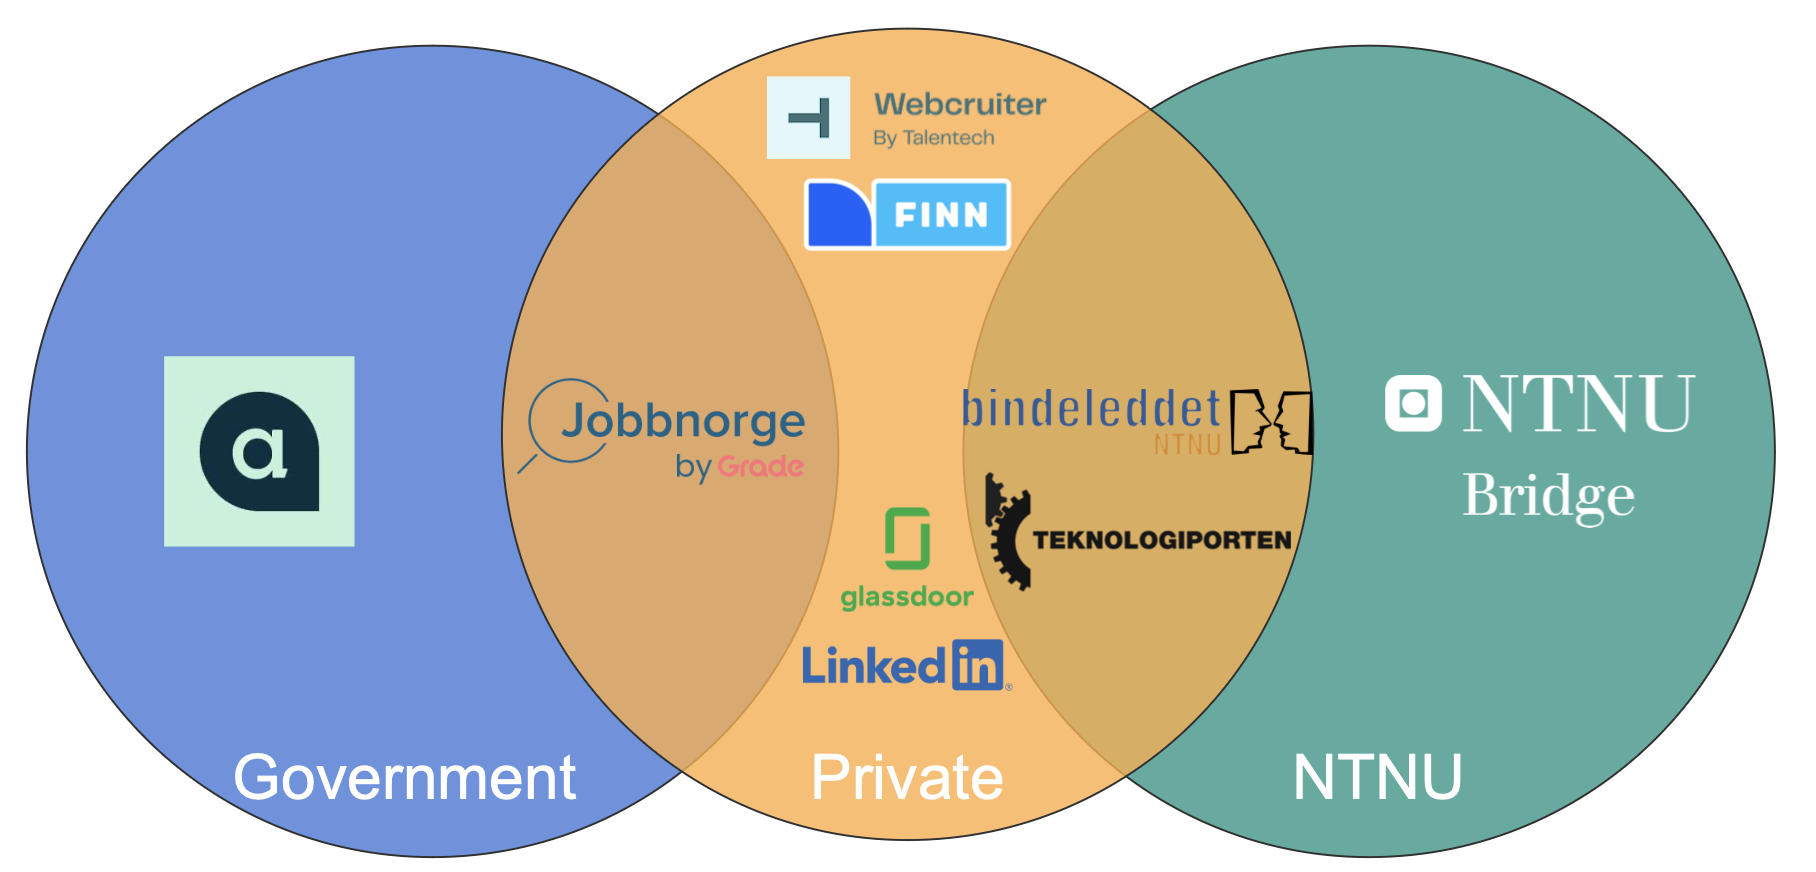
\includegraphics[width=0.8\linewidth]{images/Venn-diagram.png}
\end{figure}



\section{Finn.no}

Dette er uten tvil Norges største jobbplattform, men det handler om å bruke det smart. Inne på Finn kan man opprette nøkkelord slik at du får en varsel når jobbannonser tilknyttet disse kommer ut. Det finnes mange måter gjøre det på, men her er nøkkelordene som jeg liker å bruke:

\begin{itemize}
    \item summer intern 
    \item summer internship
    \item sommerjobb ingeniør 
    \item sommerjobb teknisk
\end{itemize}

\begin{itemize}
    \item graduate 202X
    \item nyutdannet 202X
    \item sivilingeniør
\end{itemize}

Det jeg vil anbefale er å begynne å scrolle tidlig. Jeg hadde tilfeldigvis lagret annonser fra fjoråret og da kan man se endringen fra i fjor til i år, noe som gir verdifull informasjon. Når man har lagret en annonse så er den fortsatt tilgjengelig på Finn for alle med lenken, og dette er gull verdt! Jeg har et Excel-ark som inneholder alle relevante annonser og hvis man lagrer Finn-lenken så har man likevel tilgang selv etter at det har blitt deaktivert. 


\section{LinkedIn}

LinkedIn kan beskrives som corporate versjonen av Facebook, hvor folk av og til legger ut litt kleine innlegg (og ja, jeg snakker også om meg selv). Fun fact: LinkedIn er eid av Microsoft. Av en eller annen grunn synes jeg det er utrolig gøy å klikke inn på profiler for å se hva folk driver med. Men LinkedIn er ikke bare til for nettverking – det er også en utmerket plattform for å finne jobber, noe LinkedIn tjener penger på. Akkurat som på Finn.no kan du opprette nøkkelord og sette opp varsler for stillinger som passer dine interesser. Det som skiller LinkedIn er at det er en internasjonal plattform, og større selskaper foretrekker ofte å poste stillingsannonser der fremfor på Finn.no – kanskje fordi det er billigere, men hvem vet?

\begin{remark}
    \textbf{PROTIP STALKING} Når man klikker inn på profiler på LinkedIn får vedkommende varsel om at du har vært der inne, det er kleint. Det du derimot kan gjøre er å gå inn på LinkedIn sine innstillinger og skru det av. Dette kan du ofte gjøre ved å klikke på <<Meg>>-ikonet øverst på LinkedIn-siden og deretter velge <<Innstillinger \& Personvern>> fra nedtrekksmenyen. I innstillinger og personvern, finn og klikk på <<Personvern>>-fanen som finnes langs toppen eller på siden av skjermen. Gå til <<Profilvisningsalternativer>>. Scroll ned til du finner en seksjon relatert til hvordan andre ser din aktivitet og profil, for eksempel <<Profilvisning i privatmodus>>.
\end{remark}


\section{Glassdoor}

Denne plattformen er relativt ukjent og prøver på flere måter å etterligne LinkedIn. Den brukes primært til å legge igjen anmeldelser av arbeidsgivere samt til å dele lønnsstatistikk. Informasjonen du finner der kan variere, men jeg kan dele en personlig erfaring hvor jeg hadde fått et intervju og bestemte meg for å kikke litt rundt på plattformen. Der fant jeg noen intervjuspørsmål som andre hadde delt fra samme selskap. Jeg tenkte over spørsmålet, men håpet at det ikke ville dukke opp på intervjuet – noe det selvsagt gjorde (akkurat som på en eksamen). Heldigvis var jeg forberedt siden jeg hadde vært innom Glassdoor, og den delen av intervjuet gikk bra (jeg røk dessverre ut av andre årsaker).


\section{NTNU-plattformer}

Det mange ikke vet er at det finnes en rekke plattformer som spesifikt etterspør NTNU-studenter. Disse er som følger: 

\begin{enumerate}
    \item NTNU Bridge
    \item Bindeleddet
    \item Teknologiporten
    \item HC Bedriftsider
\end{enumerate}

Jeg syntes ofte at det kan dukke opp artige stillinger på Bridge og Bindeleddet som man ellers ikke finner så kikk gjerne der også. 


\section{Karrieredager}

Det arrangeres svært mange karrieredager rundt omkring på Gløs. Her er det en liste over mange av dem og når på året det arrangeres. 

\begin{table}[H]
    \centering
    \begin{tabular}{p{2cm}p{3cm}p{7cm}}
        \toprule
        Navn & Tid & Beskrivelse \\
        \midrule
         Karrieredagene & 4 dager, starten av september & Arrangeres av Bindeleddet/indøk. Den største karrieredagen og tidlig på året. Reklameres for som om det er for hele NTNU, mens de stikker av med pengene. I 2023 var det inntekt på 3.3 mill. \cite{underdusken_tjora_karrieredagen}. \\
         IT-dagene & 2 dager, september & Arrangeres av data og komtek. \\
         Maskin- og Energidagen & 1 dag, september & Arrangeres av Maskin- og energiteknologi eller Produktutvikling og Produksjon. \\
         Kjemidagen & 1 dag, slutten av oktober & Arrangeres av nano og MTKJ. \\
         Bedriftsdagen & 1 dag, oktober & Arrangeres av marin. \\
         Energidagen & 1 dag, oktober & Arrangere av EMIL. \\
         Materialdagen & 1 dag, oktober & Arrangeres av MTMT \\
         Workation & 1 dag, okt-nov & Arrangeres av Workation, interesseorganisasjon for sommerjobb i Trondheim \\
         BM-dagen & 1 dag, starten av november & Arrangeres av bygg og miljø, inntjening på 1.8 mill. om jeg ikke har regnet feil \cite{bm_dagen_2023}. \\
         Eureka & 1 dag, januar & Arrangeres av FysMat \\
         Nettverksdagene & 3 dager, januar & Arrangeres av Kyb \\
         IV-dagene & 3 dager, februar & Av alle Ingeniørvitenskap og IKT \\
         Prospective & 2 dager, februar & Arrangeres av Teknologiporten \\
         RevolveDagen & 1 dag, februar & Arrangeres av studentorganisasjonen RevolveNTNU \\
         IAESTEs Næringslivsdager & 1 dag, mars & Av IAESTE \\
        \bottomrule
    \end{tabular}
    \caption{Oversikt over noen utvalgte karrieredager}
    \label{tab:Casekonkurranser}
\end{table}

Komplett liste finner du også på Bridge \cite{ntnu_bridge_career_days}.




\section{Svarteliste}

Denne delen er nok kontroversiell, men jeg vil påpeke at ikke alle selskaper opptrer profesjonelle til enhver tid. Det finnes mindre eksempler som det bildet under, men også noen verre eksempler jeg ønsker å påpeke.

\begin{figure}[H]
    \centering
    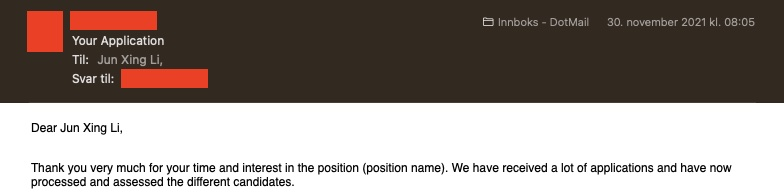
\includegraphics[width=1\linewidth]{images/mail.jpg}
\end{figure}

De verre eksemplene er mer rettet mot IT-studenter, men kan være relevant for noen fra MTKJ. Det har seg slik at noen konsulentselskaper har terminert kontrakten til sommerstudenter helt plutselig, eller permittert dem. Dette er noe som skjer i industrien under økonomisk tyngre perioder, men det er viktig å håndtere dette riktig.

\begin{figure}[H]
    \centering
    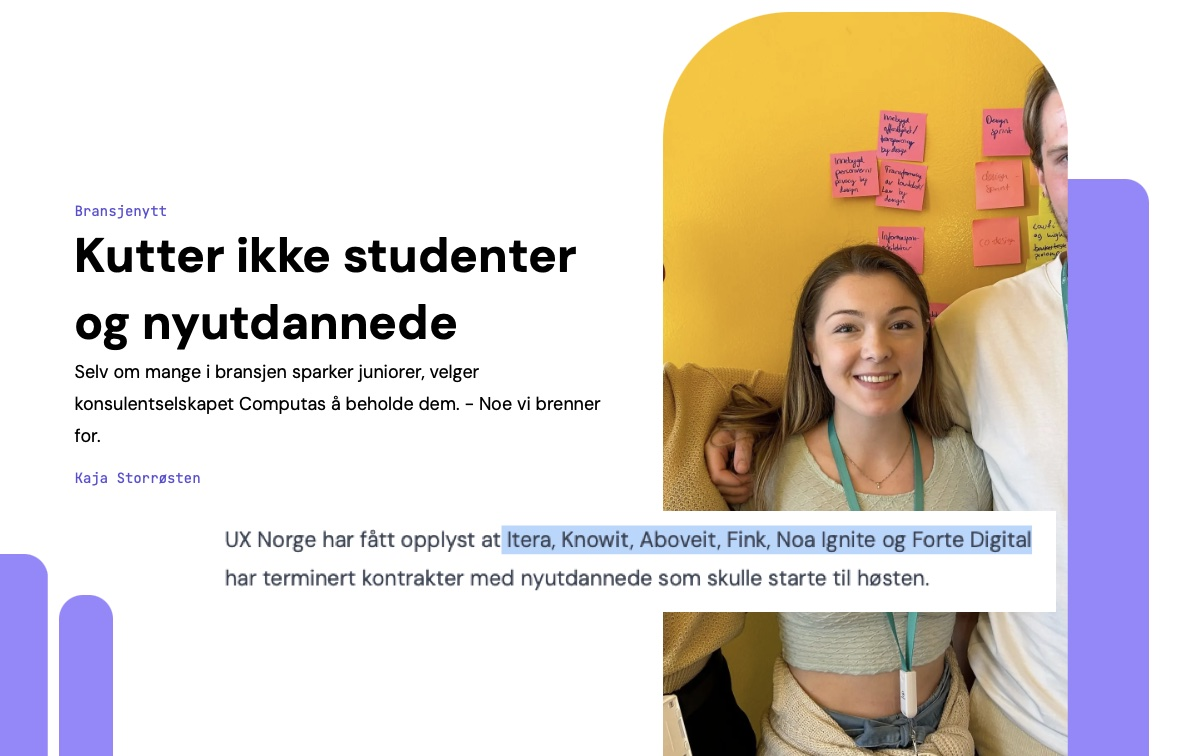
\includegraphics[width=0.8\linewidth]{images/uxnorge.jpg}
    \caption{Eksempel på hvilke selskaper som kuttet folk \cite{UXNorge2023}.}
\end{figure}

\newpage
\chapter{Intro til karriereveier}
Jeg syntes ikke at det er lett å definere de konkrete karriereveiene en fra MTKJ kan ta. Til tross for det skal jeg forsøke å snakke litt om hver av disse veiene, og her kommer sikkert mange til å være uenig med meg, men synd for deg. Noen bransjer sier seg selv, men andre er svært diffuse. Jeg tenker å starte med den mest diffuse karriereveien: konsulent. 

\section{Konsulent}

Etter min mening så finnes det hovedsakelig 3 typer konsulenter når man er utdannet som siving. ved NTNU. Disse ulike konsulentene er i realiteten svært forskjellige, men fellesnevneren er at de utenlukkende jobber for andre bedrifter ved å leie ut de ansatte. Det fører til at konsulenter kan jobbe med svært varierte prosjekter og ha mye å gjøre i gode perioder, men også at man kan ende opp med å sitte på benk i dårlige perioder (du har ingen prosjekt og tar kurs eller jobber med interne prosjekter).

\begin{figure}[H]
    \centering
    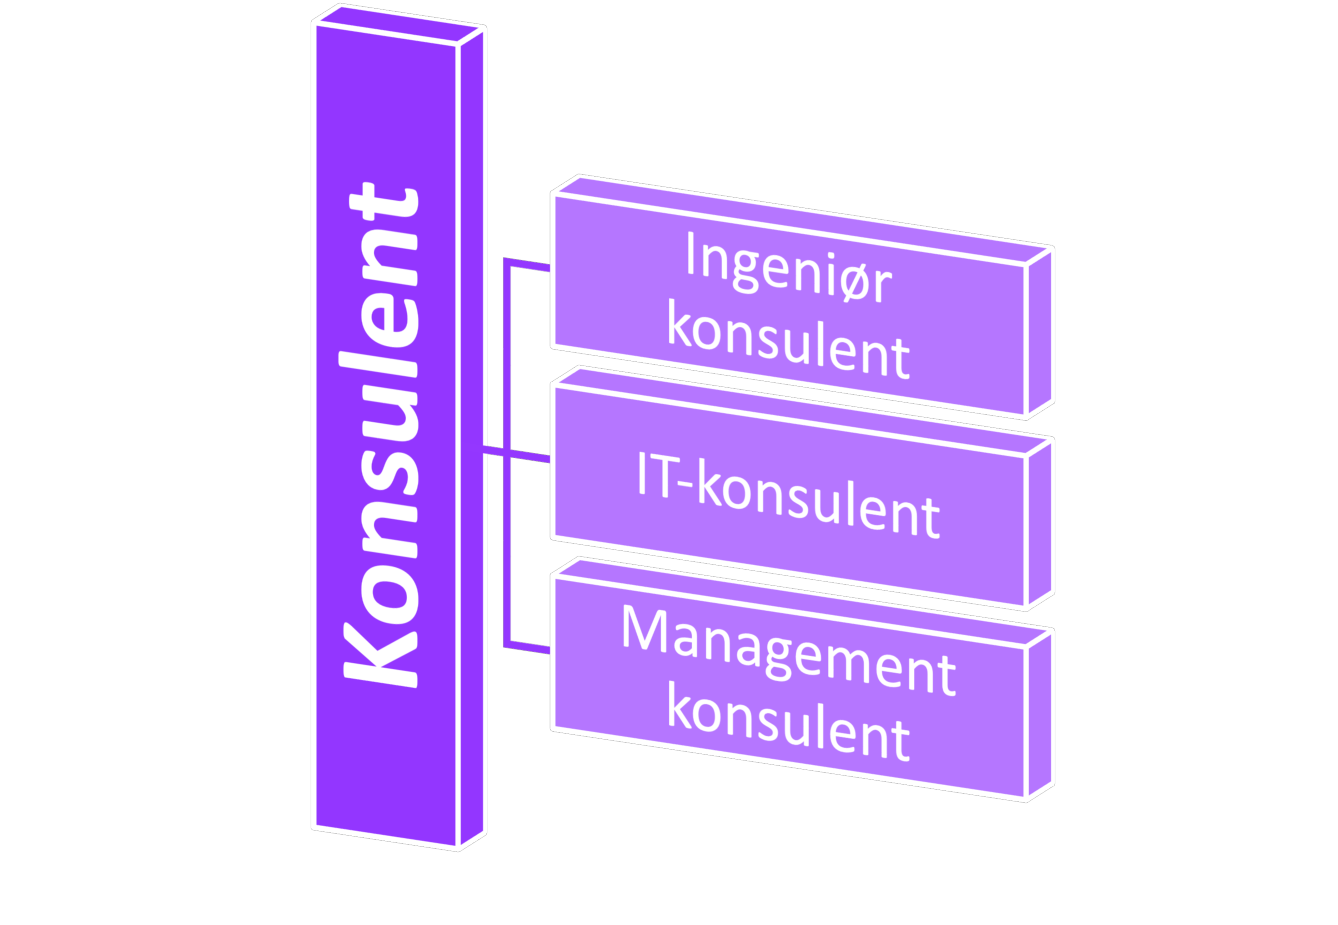
\includegraphics[width=0.5\linewidth]{images/Konsulent.pdf}
\end{figure}



\subsection{Ingeniør konsulent}

Jeg er usikker på hvor jeg har hørt dette begrepet eller om jeg fant på det selv, men en ingeniør konsulent er betegnelsen jeg velger å bruke om folk fra følgende selskaper:

\begin{figure}[H]
    \centering
    \includegraphics[width=1\linewidth]{images/Ingeniør-Konsulent.pdf}
    \caption{Oversikt over såkalte \textit{Ingeniør konsulent} bedrifter, sortert etter antall ansatte.}
    \label{fig:ingeniør-konsulent}
\end{figure}

Selskapene omtales også som bygg og anlegg ettersom disse selskapene hovedsakelig prosjekterer konstruksjoner og leier ut sine konsulenter (også kalt rådgivere). Siden mange selskaper er skandinaviske så refereres de ansatte til som rådgivere, men betydningen er det samme. Typiske oppgaver de driver med er prosjektering av karbonfangstanlegg, bygge vindparker og den type ingeniørarbeid. Denne typen konsulent er derfor mye mer teknisk og samsvarer mer med hva man studerte på Gløs enn de andre typene konsulenter. 



\subsection{IT-konsulent}

Det finnes svært mange IT-konsulentselskaper og de holder hovedsakelig på med å leie ut sine ansatte for IT-prosjekter. Disse prosjektene kan være å bygge opp et system for Equinor eller å bistå Trøndelag med Helseplattformen - Altså alt som har noe med IT å gjøre. Det er høy turnover i både IT-konsulentbransjen og managementkonsulentbransjen, noe som betyr at de ansatte typisk ikke er lenge i bransjen. Dette er fordi man kan hoppe fra prosjekt til prosjekt som IT-konsulent, hvor noen varer i uker, mens andre kan vare i måneder eller år. Det som ofte kan skje, er at man blir lei av å bytte prosjekt så ofte og mange velger derfor å heller bytte jobb til den kunden man jobber for. Grunnet høy turnover så er IT-konsulentselskaper helt rå på rekruttering. Derfor holder de masse bedpres, er veldig på med å finne graduates og kan ofte tilby heltidsjobb etter endt sommerjobb. Eksempelvis kan Sopra Steria ta imot over 200 nyutdannede og kaste dem ut i prosjekter de aldri har hold på med før. IT-konsulentbedriftene er derfor helt rå på opplæring og derfor settes det mer vekt på lærevillighet enn hva du nødvendigvis kan. Tanken er at hvis du er flink på Gløs og klarer å lære alt fra fluidmekanikk til numerisk matematikk, så klarer man å lære seg det som trengs i IT-bransjen relativt lett.

\begin{figure}[H]
    \centering
    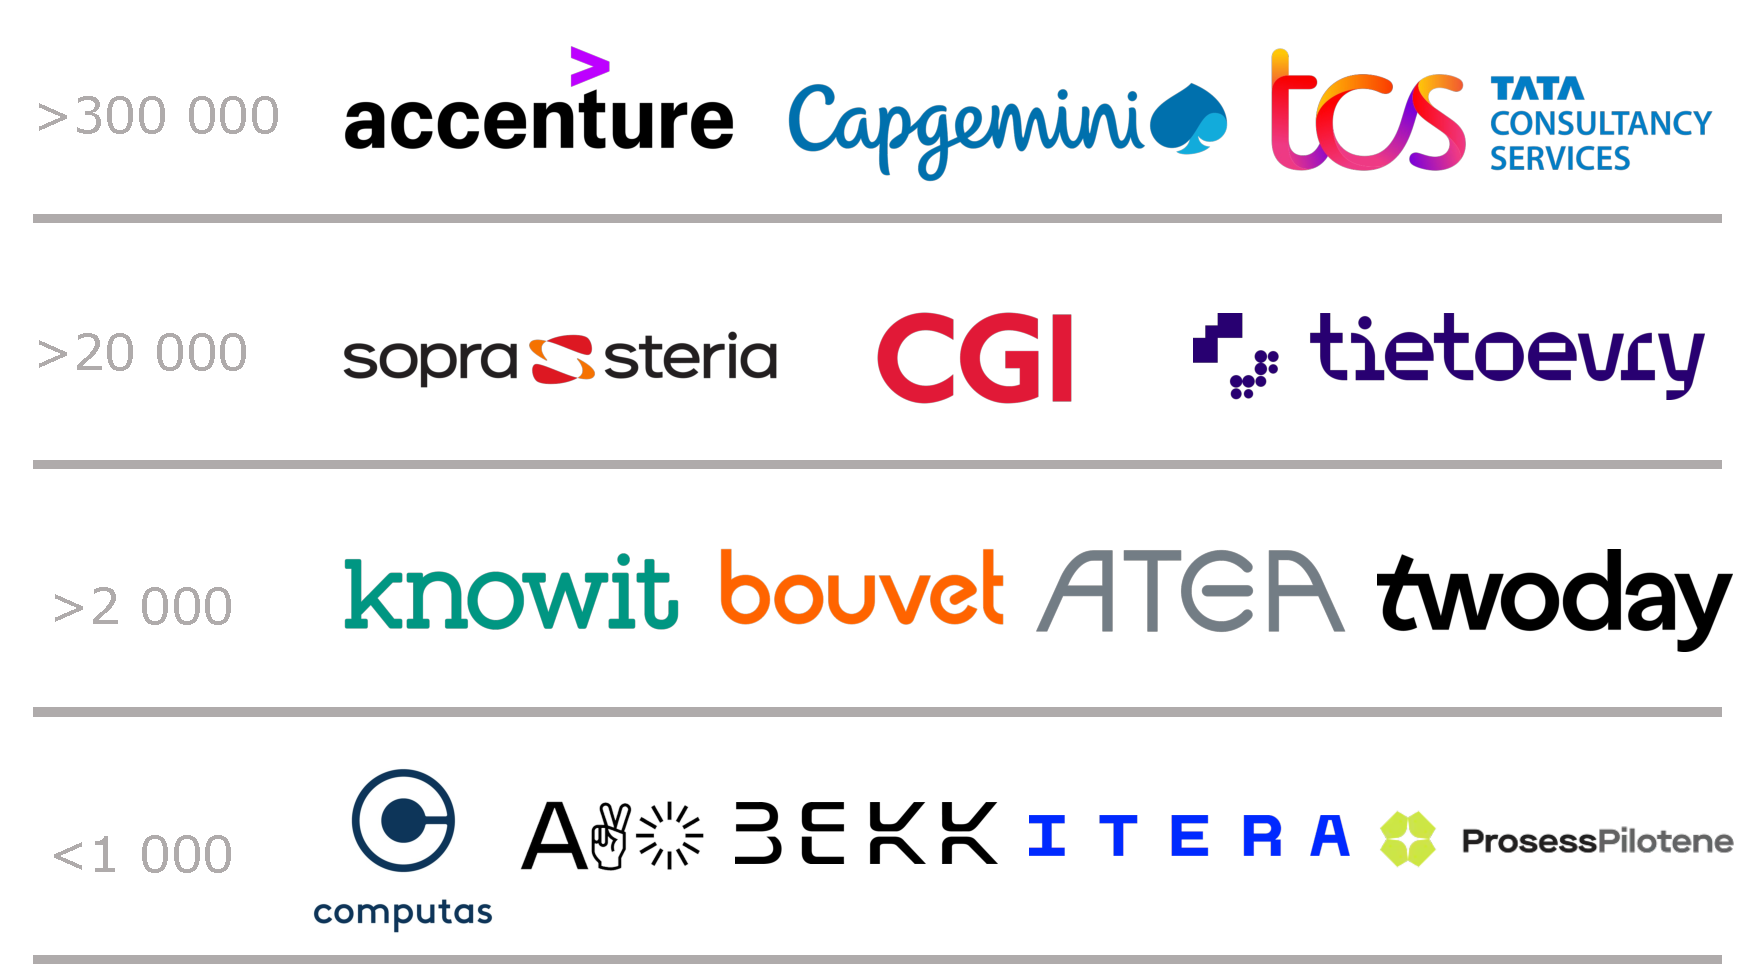
\includegraphics[width=1\linewidth]{images/IT-konsulent.pdf}
    \caption{Oversikt over utvalgte IT-konsulentselskaper, sortert etter antall ansatte.}
    \label{fig:enter-label}
\end{figure}

Listen med IT-konsulentselskaper er ikke komplett ettersom det finnes utallig mange aktører. Jeg har valgt ut noen av de som er mer kjent og av ulike størrelser. Det finnes derfor mange flere IT-konsulentselskaper enn det gjør innen bygg og anlegg. Det som også er verdt å merke seg er at disse selskapene er mye mer internasjonale, noe som fører til at størrelsen til noen av dem er helt enorme (f.eks. Accenture).



\subsection{Management konsulent}

En management konsulent kan kategoriseres som de konsulentene som verken driver med ingeniørarbeid eller direkte IT-tjenester. Det er derfor den vanskeligste rollen å definere fordi det er så mangt. Slike konsulenter ser ofte på hvilken skole du kommer fra og ikke så mye om du går EMIL eller Kyb. Derimot så er de svært ettertraktet siden både ingeniører, økonomer og samfunnsvitere kan bli management konsulenter. Derfor kan typiske arbeidsoppgaver handle om å definere selskapsstrategier eller investeringsbeslutninger osv. Du kan få en oppgave fra Posten om å definere satsningsområder, hjelpe Hafslund gjennom et oppkjøp av et annet selskap eller hjelpe en start-up med å vokse og stå på sine egne bein. 

\begin{figure}[H]
    \centering
    
\includegraphics[width=1\linewidth]{images/Manage-Konsulent.pdf}
    \caption{Oversikt over management konsulentselskaper sortert etter kategori.}
    \label{fig:enter-label}
\end{figure}

Siden slike konsulenter kan drive med så mye så deles de ofte inn i ulike kategorier som vist over. \textbf{MBB} står for \textit{McKinsey, BCG og Bain} og er anerkjent som de mest prestisjefulle konsulentselskapene å jobbe hos, også kalt for \textit{Tier 1}. De rekrutterer kun fra toppsjiktet, altså folk med toppkarakterer fra Gløs for eksempel. De er også internasjonalt anerkjent og forbindes med status. McKinsey er den største og de er veldig hemmelighetsfulle om sine kunder, men f.eks. serien \textit{Dopesick} (Disney+) handler om hvordan McKinsey-konsulenter arbeidet med Purdue Pharma for å drive salget av OxyContin, til tross for økende bevis på at medisinen var sterkt avhengighetsskapende og en drivkraft bak opioidkrisen. \textbf{Big 4}, eller de fire store, er gigantiske selskaper som hovedsakelig består av revisorer. De er med i denne oversikten ettersom denne bransjen krever at man er i kontakt med mange selskaper, så derfor driver de også med konsulenttjenester. De var tidligere mye større på konsulentsiden, men en lov fra USA, Sarbanes–Oxley Act, førte til at mange måtte selge sine konsulenttjenester. På den tiden var det faktisk Big 5, men den siste ble tatt i ulovlig shit og forsvant. PwC sine konsulenttjenester ble solgt til IBM, EY til Capgemini og KPMG til Bearingpoint. 

I motsetning til MBB som sender et fåtall konsulenter til et prosjekt, kan Big 4 sende flere titalls. Derfor kan Big 4 ofte jobbe med implementeringsprosjekter som krever mange hoder, mens MBB fokuserer mye mer på den overordnende strategien. \textbf{Lokale konsulenthus} defineres av å være norske eller skandinaviske og driver mye med det MBB holder på med, bare på et lokalt nivå. Den siste kategorien er \textbf{Spesialitet konsulenthus}, altså de som er gode på et konkret område. Eksempelvis er Rystad Energy svært gode innen energianalyse, mens Thema er gode på strømmarkedet i Norden. 

Det er verdt å nevne at siden de fleste av konsulentselskapene er utenlandske så følger de ikke-norske prinsipper. Det er eksempelvis vanlig å bli <<rangert>> eller at de setter karakter på hvor dyktig du har vært. De fleste blir satt i midten, mens de som virkelig fortjener det får topp og de som underpresterer får ofte dårligere karakterer. Dette er for å gi deg tilbakemelding på hvordan du kan bli bedre, men karakteren teller ofte på hvor mye bonus du får. Les mer på E24 \cite{e24_talentfabrikkene}.

\begin{figure}[H]
    \centering
    
\includegraphics[width=0.5\linewidth]{images/konsulent_meme.png}
\end{figure}


\section{Industri}

Det er lett for meg å kategorisere karriereveier som enten konsulent eller industri, men sånn får det bli. Poenget er at disse industribedriftene jobber med ganske konkrete ting, som sier seg selv, mens konsulentene krever mer forklaring. Det finnes et betydelig antall fra MTKJ som jobber i konsulentbransjen, men det er absolutt flest innen industrien. Derfor vil følgende liste med bedrifter være en god representasjon av karriereveier (jeg tør å påstå at 90\% av MTKJ-ere er i disse selskapene).

\begin{figure}[H]
    \centering
    
\includegraphics[width=1\linewidth]{images/Industri1.pdf}
    \caption{Industri, del 1}
    \label{fig:industri1}
\end{figure}

\textbf{Oljeselskaper} kjenner nok de fleste til. De driver gjerne med utvinning av olje og gass. \textbf{Oljeservice selskaper} derimot, jobber tett mot oljeselskapene og kan bistå med bygging og ulike tekniske løsninger. For eksempel så er Aker BP operatør, mens Aker Solutions bistår med alt annet rundt. \textbf{Metallindustri} sier også seg selv med at de produserer metaller. Hydro produserer aluminium, Eramet produserer ferromangan osv. I Norge er det veldig mange slike selskaper, men de ligger ofte langt fra store byer. \textbf{Kjemisk industri} produserer derimot kjemiske produkter og her er spennet svært bredt. Det kan være røntgenkontrastmidler fra GE Healthcare til gjødsel fra Yara. 

\begin{figure}[H]
    \centering
    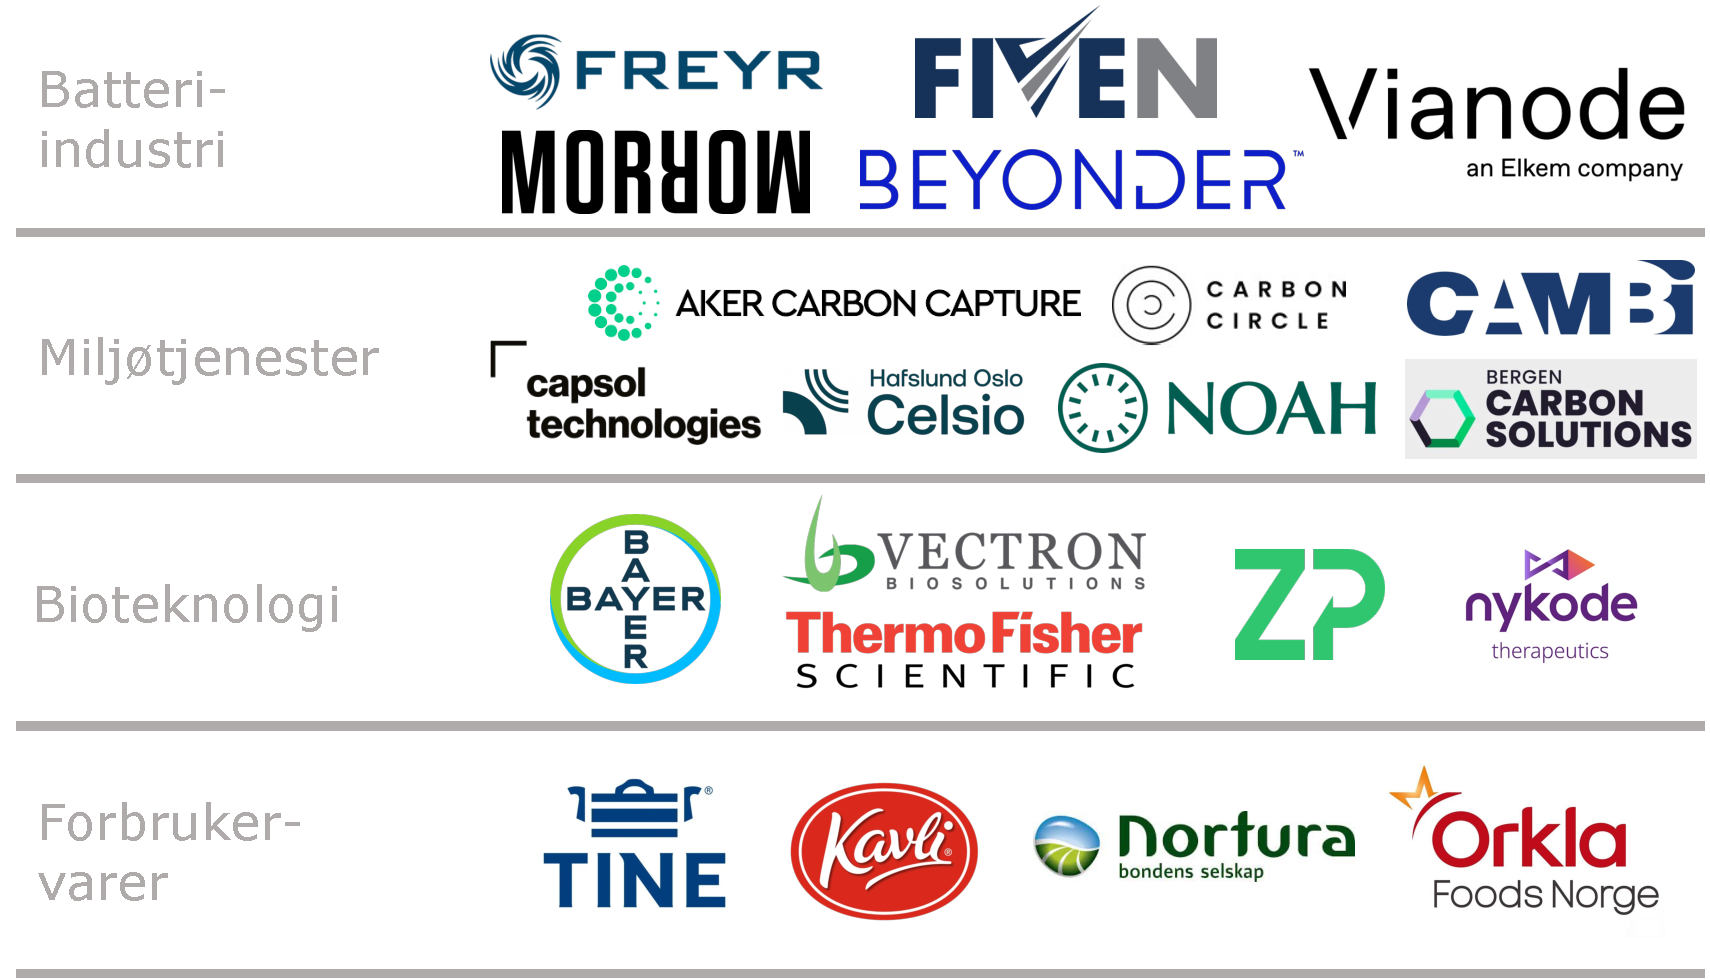
\includegraphics[width=1\linewidth]{images/Industri2.pdf}
    \caption{Industri, del 2}
    \label{fig:industri2}
\end{figure}

Den neste kategorien er \textbf{batteriindustri}, og den sier også seg selv da de produserer batterier, men dette er en relativ ny industri i Norge og derav under konstant utvikling. \textbf{Miljøtjenester} har jeg kalt selskaper som jobber med alt fra karbonfangst til avfallshåndtering. \textbf{Bioteknologi} har jeg kalt de som driver med medisinsk forskning og sånt. \textbf{Forbrukervarer} trenger jeg ikke å forklare.

\begin{figure}[H]
    \centering
    
\includegraphics[width=1\linewidth]{images/Industri3.pdf}
    \caption{Industri, del 3}
    \label{fig:industri3}
\end{figure}

\textbf{Industriell IT} har jeg kalt de som utelukkende bistår industrien med IT-løsninger. Cognite eies av Aker og driver med masse fancy maskinlæring til Aker BP.
\textbf{Forskning} er kanskje feil å kategorisere som en industri, men det får gå. Her er det verdt å merke at det er en vesentlig forskjell mellom NTNU og f.eks. SINTEF ettersom SINTEF er et privat selskap, mens NTNU er offentlig. Derfor er det store forskjeller innad i denne kategorien. \textbf{Trainee} er en kategori som består av ulike traineepropgram overalt i Norge. Mange selskaper har opplegg hvor man roterer mellom avdelinger, mens disse traineeprogrammene er mellom ulike selskaper. De finnes ofte for å tiltrekke seg unge til mindre ettertraktede steder. \textbf{Havbruk} jobber med fisk og den verdikjeden der da, ellernoe sånt. 

\begin{figure}[H]
    \centering
    
\includegraphics[width=1\linewidth]{images/Industri4.pdf}
    \caption{Industri, del 4}
    \label{fig:industri4}
\end{figure}

\textbf{Våpen} lager jo, våpen. Og den siste kategorien \textbf{Andre} er de jeg ikke klarer å få til å passe inn i eksisterende kategorier. Norcem lager sement, men det er jo ikke direkte kjemisk industri? DNV driver med standarder og regelverk, passer jo heller ikke inn i de andre. 

\newpage
\chapter{Lønn}
\input{sections/part2/3.Lønn}

\newpage
\chapter{Tips til CV og søknad}
\input{sections/part2/4.Tips til CV og søknad}

\newpage
\part{Referanser}
\printbibliography[title={Referanser}] %you may change the title in the toc here if you want
\end{document}
